\documentclass[11pt, letterpaper]{article}

% Fonts and Encoding
\usepackage[utf8]{inputenc}
\usepackage[T1]{fontenc}
\usepackage{lmodern} % High-quality Latin Modern vector font

% Math and Symbols
\usepackage{amsmath, amssymb, amsthm, amsfonts, mathrsfs, mathtools}

% Layout and Geometry
\usepackage{geometry}
\geometry{letterpaper, margin=1in}
\setlength{\parindent}{0pt}
\setlength{\parskip}{0.6em}

% Formatting and Graphics
\usepackage{graphicx, xcolor, enumitem, booktabs, array, tabularx}

% TikZ for Illustrations
\usepackage{tikz}
\usetikzlibrary{arrows.meta, positioning, shapes.geometric, calc, backgrounds, matrix}

% Clickable Links and TOC
\usepackage{hyperref}
\hypersetup{
    colorlinks=true,
    linkcolor=blue,
    filecolor=magenta,      
    urlcolor=cyan,
    pdftitle={Least-Squares Problems: Comprehensive Problem Set and Detailed Solutions},
}

% Theorem Environments
\newtheorem{theorem}{Theorem}[section]
\newtheorem{lemma}[theorem]{Lemma}
\newtheorem{proposition}[theorem]{Proposition}
\newtheorem{corollary}[theorem]{Corollary}
\theoremstyle{definition}
\newtheorem{definition}{Definition}[section]
\newtheorem{axiom}{Axiom}[section]
\newtheorem{example}{Example}[section]
\theoremstyle{remark}
\newtheorem{remark}{Remark}[section]

% Custom Commands (Enforced standard notation)
\newcommand{\R}{\mathbb{R}}
\newcommand{\N}{\mathbb{N}}
\newcommand{\Z}{\mathbb{Z}}
\newcommand{\Q}{\mathbb{Q}}
\newcommand{\E}{\mathbb{E}}
\newcommand{\Prob}{\mathbb{P}}
\newcommand{\F}{\mathcal{F}}

\title{Least-Squares Problems: Comprehensive Problem Set and Detailed Solutions}
\author{Tashfeen Omran}
\date{\today}

\begin{document}

\maketitle
\tableofcontents
\newpage

\section{Concept Checklist and Question Mapping}

This guide provides a comprehensive mastery set of 31 problems covering Section 6.5 (Least-Squares Problems), spanning computational methods, orthogonal projections, singular normal equations, $QR$ factorization, Tikhonov regularization (Ridge Regression), quantitative finance and machine learning applications, theoretical proofs, and diagnostic flaw detection.

\subsection{Visualizing the Least-Squares Projection}

When an overdetermined system $A\mathbf{x} = \mathbf{b}$ is inconsistent ($\mathbf{b} \notin \operatorname{Col} A$), the least-squares solution $\hat{\mathbf{x}} \in \mathbb{R}^n$ produces the vector $\hat{\mathbf{b}} = A\hat{\mathbf{x}} \in \operatorname{Col} A$ that is closest to $\mathbf{b} \in \mathbb{R}^m$. Geometrically, $\hat{\mathbf{b}}$ is the orthogonal projection of $\mathbf{b}$ onto $\operatorname{Col} A$, and the residual vector $\mathbf{b} - A\hat{\mathbf{x}}$ is orthogonal to every column of $A$.

\begin{center}
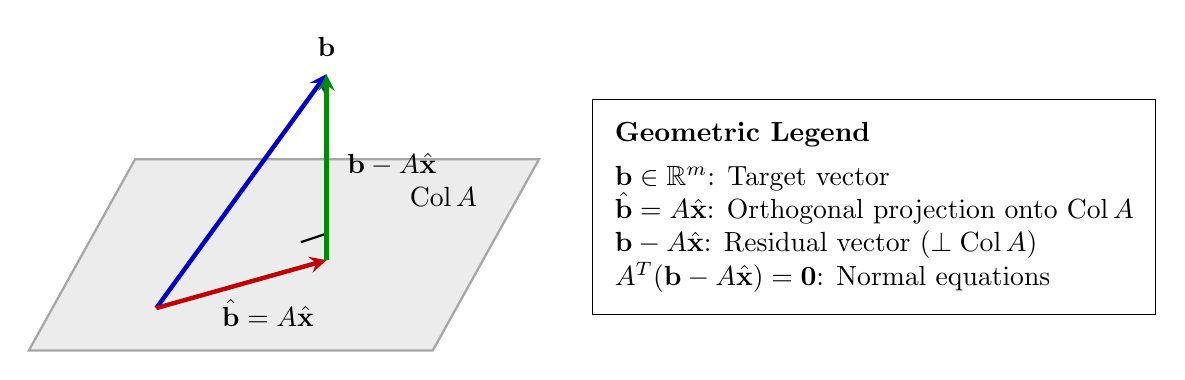
\begin{tikzpicture}[scale=1.35]
    % Layer 1: Background subspace fill
    \fill[gray!15] (0,0) -- (3.8,0) -- (4.8,1.8) -- (1.0,1.8) -- cycle;

    % Layer 2: Subspace boundary and right-angle geometry
    \draw[gray!70, thick] (0,0) -- (3.8,0) -- (4.8,1.8) -- (1.0,1.8) -- cycle;
    \draw[black, thick] (2.8,0.85) -- (2.8,1.1) -- (2.56,1.02);

    % Layer 3: Primary vectors
    \draw[->, >=stealth, ultra thick, blue!80!black] (1.2,0.4) -- (2.8,2.6);
    \draw[->, >=stealth, ultra thick, red!75!black] (1.2,0.4) -- (2.8,0.85);
    \draw[->, >=stealth, ultra thick, green!55!black] (2.8,0.85) -- (2.8,2.6);

    % Layer 4: Text labels and off-axis single-node multiline legend
    \node[black, above=3pt] at (2.8,2.6) {$\displaystyle \mathbf{b}$};
    \node[black, below=3pt] at (2.25,0.65) {$\displaystyle \hat{\mathbf{b}} = A\hat{\mathbf{x}}$};
    \node[black, right=4pt] at (2.8,1.75) {$\displaystyle \mathbf{b} - A\hat{\mathbf{x}}$};
    \node[black] at (3.9,1.45) {$\operatorname{Col} A$};

    \node[anchor=west, align=left, draw=black, fill=white, inner sep=8pt, text=black] at (5.3,1.35) {%
        \textbf{Geometric Legend}\\[4pt]
        $\mathbf{b} \in \mathbb{R}^m$: Target vector\\
        $\hat{\mathbf{b}} = A\hat{\mathbf{x}}$: Orthogonal projection onto $\operatorname{Col} A$\\
        $\mathbf{b} - A\hat{\mathbf{x}}$: Residual vector ($\perp \operatorname{Col} A$)\\
        $A^T(\mathbf{b} - A\hat{\mathbf{x}}) = \mathbf{0}$: Normal equations
    };
\end{tikzpicture}
\end{center}

\subsection{Problem Types and General Approach}

\begin{description}
    \item[Concept 1: Basic Normal Equations (Assigned: Problems 1--3)] \hfill \\
    \textbf{Problem Archetype:} Finding the unique least-squares solution $\hat{\mathbf{x}}$ of an inconsistent system $A\mathbf{x} = \mathbf{b}$ when the columns of $A$ are linearly independent.\\
    \textbf{Strategic Workflow:}
    \begin{itemize}
        \item Compute the symmetric $n \times n$ matrix $A^T A$ and the vector $A^T \mathbf{b}$ (never $AA^T$).
        \item Form the normal equations $A^T A \hat{\mathbf{x}} = A^T \mathbf{b}$.
        \item If $A^T A$ is $2 \times 2$, solve via the inverse formula $\hat{\mathbf{x}} = (A^T A)^{-1} A^T \mathbf{b}$ or elimination; for $3 \times 3$ or larger, apply Gaussian elimination on $[A^T A \mid A^T \mathbf{b}]$.
    \end{itemize}

    \item[Concept 2: Orthogonal Projection and Least-Squares Error (Assigned: Problems 4--6)] \hfill \\
    \textbf{Problem Archetype:} Computing the closest vector $\hat{\mathbf{b}} \in \operatorname{Col} A$ to $\mathbf{b}$, verifying residual orthogonality, and finding the minimum distance $\|\mathbf{b} - A\hat{\mathbf{x}}\|$.\\
    \textbf{Strategic Workflow:}
    \begin{itemize}
        \item Solve the normal equations $A^T A \hat{\mathbf{x}} = A^T \mathbf{b}$ for the weight vector $\hat{\mathbf{x}} \in \mathbb{R}^n$.
        \item Compute the orthogonal projection $\hat{\mathbf{b}} = A\hat{\mathbf{x}} \in \mathbb{R}^m$ (do not confuse $\hat{\mathbf{x}}$ with $\hat{\mathbf{b}}$).
        \item Compute the residual vector $\mathbf{r} = \mathbf{b} - \hat{\mathbf{b}}$, check $A^T \mathbf{r} = \mathbf{0}$, and compute the error $\|\mathbf{b} - \hat{\mathbf{b}}\| = \sqrt{(\mathbf{b} - \hat{\mathbf{b}})^T(\mathbf{b} - \hat{\mathbf{b}})}$.
    \end{itemize}

    \item[Concept 3: Infinite Least-Squares Solutions (Assigned: Problems 7--10)] \hfill \\
    \textbf{Problem Archetype:} Describing the entire family of least-squares solutions when the columns of $A$ are linearly dependent (making $A^T A$ singular), including finding the minimum-norm least-squares solution.\\
    \textbf{Strategic Workflow:}
    \begin{itemize}
        \item Compute $A^T A$ and $A^T \mathbf{b}$, noting that $\det(A^T A) = 0$ implies non-uniqueness, not inconsistency.
        \item Form the augmented matrix $[A^T A \mid A^T \mathbf{b}]$ and row reduce to Reduced Row Echelon Form (RREF).
        \item Express the general solution $\hat{\mathbf{x}}$ in parametric vector form using free variables, and note that $\hat{\mathbf{b}} = A\hat{\mathbf{x}}$ remains unique.
    \end{itemize}

    \item[Concept 4: Orthogonal Columns Shortcut (Assigned: Problems 11--13)] \hfill \\
    \textbf{Problem Archetype:} Solving $A\mathbf{x} = \mathbf{b}$ or tuning parameters so that the columns $\mathbf{a}_1, \dots, \mathbf{a}_n$ of $A$ are mutually orthogonal, decoupling the normal equations.\\
    \textbf{Strategic Workflow:}
    \begin{itemize}
        \item Explicitly verify $\mathbf{a}_i \cdot \mathbf{a}_j = 0$ for all $i \neq j$.
        \item Use the resulting diagonal structure of $A^T A$ to compute each weight independently via $\hat{x}_i = \frac{\mathbf{a}_i \cdot \mathbf{b}}{\mathbf{a}_i \cdot \mathbf{a}_i}$.
        \item Compute $\hat{\mathbf{b}} = \sum_{i=1}^n \frac{\mathbf{a}_i \cdot \mathbf{b}}{\mathbf{a}_i \cdot \mathbf{a}_i}\mathbf{a}_i$.
    \end{itemize}

    \item[Concept 5: $QR$ Factorization Method (Assigned: Problems 14--17)] \hfill \\
    \textbf{Problem Archetype:} Solving least-squares problems using $A = QR$ (either given $Q, R$ or after constructing them via Gram--Schmidt) to avoid the numerical instability of forming $A^T A$.\\
    \textbf{Strategic Workflow:}
    \begin{itemize}
        \item Avoid computing $A^T A$ or $R^{-1}$.
        \item Compute the vector $Q^T \mathbf{b}$.
        \item Solve the upper triangular system $R\hat{\mathbf{x}} = Q^T \mathbf{b}$ via back-substitution from the bottom row upward.
        \item When asked for $\hat{\mathbf{b}}$, compute $\hat{\mathbf{b}} = Q(Q^T \mathbf{b})$.
    \end{itemize}

    \item[Concept 6: Tikhonov Regularization and Ridge Regression (Assigned: Problems 18--20)] \hfill \\
    \textbf{Problem Archetype:} Stabilizing ill-conditioned or singular normal equations caused by multicollinearity via an $L_2$ penalty parameter $\lambda > 0$.\\
    \textbf{Strategic Workflow:}
    \begin{itemize}
        \item Form $A^T A$ and check its determinant or conditioning.
        \item Add $\lambda I$ to the diagonal to obtain the modified normal equations $(A^T A + \lambda I)\hat{\mathbf{x}}_{\text{ridge}} = A^T \mathbf{b}$.
        \item Solve the strictly positive definite system to obtain shrunk, stable coefficient estimates.
    \end{itemize}

    \item[Concept 7: Applied Modeling in Finance and Machine Learning (Assigned: Problems 21--23)] \hfill \\
    \textbf{Problem Archetype:} Formulating and solving Ordinary Least Squares (OLS) estimators for multi-factor asset pricing ($\mathbf{r} = F\boldsymbol{\beta} + \boldsymbol{\epsilon}$) and linear regression models.\\
    \textbf{Strategic Workflow:}
    \begin{itemize}
        \item Construct the design matrix ($F$ or $X$, including a column of ones if an intercept is present) and target vector.
        \item Compute $\hat{\boldsymbol{\beta}} = (F^T F)^{-1} F^T \mathbf{r}$ via the normal equations.
        \item Compute predicted targets, residuals, and Mean Squared Error ($\text{MSE} = \frac{1}{m}\|\mathbf{y} - X\hat{\mathbf{w}}\|^2$).
    \end{itemize}

    \item[Concept 8: Theoretical Proofs and Matrix Properties (Assigned: Problems 24--26)] \hfill \\
    \textbf{Problem Archetype:} Proving foundational theorems regarding $\operatorname{Nul} A = \operatorname{Nul}(A^T A)$, invertibility of $A^T A$, consistency of normal equations, uniqueness of $\hat{\mathbf{b}}$, gradient derivations, and properties of projection matrices.\\
    \textbf{Strategic Workflow:}
    \begin{itemize}
        \item Apply the transpose distribution trick: $\mathbf{x}^T A^T A \mathbf{x} = (A\mathbf{x})^T(A\mathbf{x}) = \|A\mathbf{x}\|^2$.
        \item Use the Orthogonal Decomposition Theorem ($\mathbb{R}^m = \operatorname{Col} A \oplus \operatorname{Nul} A^T$).
        \item Use matrix calculus identities $\nabla_{\mathbf{x}}(\mathbf{c}^T \mathbf{x}) = \mathbf{c}$ and $\nabla_{\mathbf{x}}(\mathbf{x}^T M \mathbf{x}) = 2M\mathbf{x}$ for symmetric $M$.
    \end{itemize}

    \item[Concept 9: Diagnostic Analysis: Find the Flaw (Assigned: Problems 27--31)] \hfill \\
    \textbf{Problem Archetype:} Auditing flawed least-squares work to diagnose critical conceptual errors ($AA^T$ order, $\|\mathbf{b}-\hat{\mathbf{x}}\|$, $R^T$ mix-up, non-orthogonal column shortcut, and false non-existence when $\det(A^T A)=0$).\\
    \textbf{Strategic Workflow:}
    \begin{itemize}
        \item Check matrix dimensions, transposition order, orthogonality prerequisites, and invertibility assumptions step by step.
        \item Explain precisely why the flawed step violates linear algebra theorems.
        \item Recompute the problem from scratch using the valid method.
    \end{itemize}
\end{description}

\newpage

\section{Problem Sets}

\subsection{Basic Normal Equations}

\textbf{Problem 1.} Find the least-squares solution $\hat{\mathbf{x}}$ of $A\mathbf{x} = \mathbf{b}$ by (a) constructing the normal equations for $\hat{\mathbf{x}}$ and (b) solving for $\hat{\mathbf{x}}$, where
\[
A = \begin{bmatrix} 1 & 3 \\ 2 & -1 \\ -1 & 2 \end{bmatrix}, \quad \mathbf{b} = \begin{bmatrix} 5 \\ 1 \\ 0 \end{bmatrix}.
\]

\textbf{Problem 2.} Find a least-squares solution $\hat{\mathbf{x}}$ of $A\mathbf{x} = \mathbf{b}$ for the $4 \times 2$ system
\[
A = \begin{bmatrix} 1 & -1 \\ -1 & 3 \\ 0 & 2 \\ 2 & 1 \end{bmatrix}, \quad \mathbf{b} = \begin{bmatrix} 4 \\ 2 \\ 4 \\ 2 \end{bmatrix}.
\]

\textbf{Problem 3.} Set up the normal equations and use Gaussian elimination to find the least-squares solution $\hat{\mathbf{x}}$ of $A\mathbf{x} = \mathbf{b}$, where
\[
A = \begin{bmatrix} 1 & 0 & 1 \\ 1 & 1 & 0 \\ 0 & 1 & 1 \\ 1 & 1 & 1 \end{bmatrix}, \quad \mathbf{b} = \begin{bmatrix} 2 \\ 1 \\ 3 \\ 6 \end{bmatrix}.
\]

\subsection{Orthogonal Projection and Least-Squares Error}

\textbf{Problem 4.} For the matrix $A$ and vector $\mathbf{b}$ given below, find (a) the least-squares solution $\hat{\mathbf{x}}$, (b) the orthogonal projection $\hat{\mathbf{b}} = A\hat{\mathbf{x}}$ of $\mathbf{b}$ onto $\operatorname{Col} A$, and (c) the least-squares error $\|\mathbf{b} - A\hat{\mathbf{x}}\|$:
\[
A = \begin{bmatrix} 1 & 1 \\ 1 & -1 \\ 1 & 1 \end{bmatrix}, \quad \mathbf{b} = \begin{bmatrix} 3 \\ 1 \\ 5 \end{bmatrix}.
\]

\textbf{Problem 5.} Find the closest point $\hat{\mathbf{b}}$ in $\operatorname{Col} A$ to $\mathbf{b}$ and determine the minimum distance $\|\mathbf{b} - \hat{\mathbf{b}}\|$, where
\[
A = \begin{bmatrix} 2 \\ -1 \\ 2 \end{bmatrix}, \quad \mathbf{b} = \begin{bmatrix} 5 \\ 2 \\ -1 \end{bmatrix}.
\]

\textbf{Problem 6.} Given
\[
A = \begin{bmatrix} 1 & 1 \\ 1 & 2 \\ 1 & 0 \\ 1 & 1 \end{bmatrix}, \quad \mathbf{b} = \begin{bmatrix} 3 \\ 5 \\ 1 \\ 7 \end{bmatrix},
\]
find $\hat{\mathbf{x}}$, compute the orthogonal projection $\hat{\mathbf{b}} = A\hat{\mathbf{x}}$, verify explicitly that $\mathbf{b} - \hat{\mathbf{b}}$ is orthogonal to $\operatorname{Col} A$, and compute the least-squares error $\|\mathbf{b} - \hat{\mathbf{b}}\|$.

\subsection{Infinite Least-Squares Solutions}

\textbf{Problem 7.} Describe all least-squares solutions of the equation $A\mathbf{x} = \mathbf{b}$ in parametric vector form, where
\[
A = \begin{bmatrix} 1 & 0 & 1 \\ 1 & 0 & 1 \\ 1 & 1 & 0 \\ 1 & 1 & 0 \end{bmatrix}, \quad \mathbf{b} = \begin{bmatrix} 4 \\ 2 \\ 1 \\ 5 \end{bmatrix}.
\]

\textbf{Problem 8.} Find the general least-squares solution of $A\mathbf{x} = \mathbf{b}$ and verify that every solution in the family produces the same orthogonal projection $\hat{\mathbf{b}}$, where
\[
A = \begin{bmatrix} 1 & -2 \\ 2 & -4 \\ -1 & 2 \end{bmatrix}, \quad \mathbf{b} = \begin{bmatrix} 3 \\ 5 \\ 1 \end{bmatrix}.
\]

\textbf{Problem 9.} Describe all least-squares solutions of $A\mathbf{x} = \mathbf{b}$, where
\[
A = \begin{bmatrix} 1 & 2 & 3 \\ 0 & 1 & 1 \\ 1 & 1 & 2 \end{bmatrix}, \quad \mathbf{b} = \begin{bmatrix} 4 \\ 2 \\ 0 \end{bmatrix}.
\]

\textbf{Problem 10.} Find all least-squares solutions of $A\mathbf{x} = \mathbf{b}$ for
\[
A = \begin{bmatrix} 1 & 1 & 2 \\ 1 & -1 & 0 \\ 1 & 1 & 2 \\ 1 & -1 & 0 \end{bmatrix}, \quad \mathbf{b} = \begin{bmatrix} 3 \\ 1 \\ 5 \\ -1 \end{bmatrix},
\]
and then find the unique least-squares solution $\hat{\mathbf{x}}_{\min}$ that has the smallest Euclidean norm $\|\hat{\mathbf{x}}\|$.

\subsection{Orthogonal Columns Shortcut}

\textbf{Problem 11.} Verify that the columns of $A$ are orthogonal, and use the orthogonal columns shortcut to find (a) the least-squares solution $\hat{\mathbf{x}}$ of $A\mathbf{x} = \mathbf{b}$ and (b) the orthogonal projection $\hat{\mathbf{b}}$ of $\mathbf{b}$ onto $\operatorname{Col} A$:
\[
A = \begin{bmatrix} 2 & 1 \\ -1 & 4 \\ 2 & 1 \end{bmatrix}, \quad \mathbf{b} = \begin{bmatrix} 3 \\ 1 \\ 5 \end{bmatrix}.
\]

\textbf{Problem 12.} Verify that the columns of $A$ form an orthogonal set, and use this property to find the least-squares solution $\hat{\mathbf{x}}$, the orthogonal projection $\hat{\mathbf{b}}$, and the least-squares error $\|\mathbf{b} - \hat{\mathbf{b}}\|$ for
\[
A = \begin{bmatrix} 1 & 1 & 1 \\ 1 & 1 & -1 \\ 1 & -1 & 1 \\ 1 & -1 & -1 \end{bmatrix}, \quad \mathbf{b} = \begin{bmatrix} 8 \\ 0 \\ 2 \\ 2 \end{bmatrix}.
\]

\textbf{Problem 13.} Determine the value of the scalar $k$ that makes the columns of $A$ orthogonal. For that value of $k$, use the orthogonal columns shortcut to find $\hat{\mathbf{x}}$, $\hat{\mathbf{b}}$, and $\|\mathbf{b} - \hat{\mathbf{b}}\|$ for
\[
A = \begin{bmatrix} 1 & 2 \\ 2 & k \\ 2 & 1 \end{bmatrix}, \quad \mathbf{b} = \begin{bmatrix} 4 \\ 1 \\ 5 \end{bmatrix}.
\]

\subsection{$QR$ Factorization Method}

\textbf{Problem 14.} Use the factorization $A = QR$ to find the least-squares solution $\hat{\mathbf{x}}$ of $A\mathbf{x} = \mathbf{b}$, where
\[
A = \begin{bmatrix} 1 & 4 \\ 2 & 5 \\ 2 & 2 \end{bmatrix} = \begin{bmatrix} 1/3 & 2/3 \\ 2/3 & 1/3 \\ 2/3 & -2/3 \end{bmatrix} \begin{bmatrix} 3 & 6 \\ 0 & 3 \end{bmatrix}, \quad \mathbf{b} = \begin{bmatrix} 8 \\ 4 \\ 1 \end{bmatrix}.
\]

\textbf{Problem 15.} A matrix $A$ has a $QR$ factorization $A = QR$ with
\[
R = \begin{bmatrix} 2 & -1 & 3 \\ 0 & 4 & 2 \\ 0 & 0 & -5 \end{bmatrix}, \quad \text{and} \quad Q^T \mathbf{b} = \begin{bmatrix} 10 \\ 4 \\ 10 \end{bmatrix}.
\]
Find the least-squares solution $\hat{\mathbf{x}}$ of $A\mathbf{x} = \mathbf{b}$ without computing $A$ or $A^T A$.

\textbf{Problem 16.} Compute the $QR$ factorization of $A$ via the Gram--Schmidt process, and use $R\hat{\mathbf{x}} = Q^T \mathbf{b}$ to find the least-squares solution of $A\mathbf{x} = \mathbf{b}$ for
\[
A = \begin{bmatrix} 1 & 2 \\ 1 & 0 \\ 1 & 2 \\ 1 & 0 \end{bmatrix}, \quad \mathbf{b} = \begin{bmatrix} 6 \\ 2 \\ 2 \\ 0 \end{bmatrix}.
\]

\textbf{Problem 17.} A $4 \times 2$ matrix $A$ has the $QR$ factorization
\[
A = \begin{bmatrix} 1/2 & 1/2 \\ 1/2 & 1/2 \\ 1/2 & -1/2 \\ 1/2 & -1/2 \end{bmatrix} \begin{bmatrix} 2 & 4 \\ 0 & 6 \end{bmatrix}, \quad \text{and} \quad \mathbf{b} = \begin{bmatrix} 7 \\ 3 \\ 1 \\ 5 \end{bmatrix}.
\]
Use the $QR$ factorization to find (a) the least-squares solution $\hat{\mathbf{x}}$, (b) the orthogonal projection $\hat{\mathbf{b}} = Q(Q^T \mathbf{b})$, and (c) the least-squares error $\|\mathbf{b} - \hat{\mathbf{b}}\|$.

\subsection{Tikhonov Regularization and Ridge Regression}

\textbf{Problem 18.} Consider the ill-conditioned system $A\mathbf{x} = \mathbf{b}$ with nearly collinear columns:
\[
A = \begin{bmatrix} 1 & 1 \\ 1 & 1.02 \\ 1 & 1 \end{bmatrix}, \quad \mathbf{b} = \begin{bmatrix} 2 \\ 4 \\ 2 \end{bmatrix}.
\]
(a) Compute $A^T A$ and its determinant. (b) Apply Ridge Regression with $\lambda = 0.1$ to compute $A^T A + \lambda I$ and its determinant. (c) Solve $(A^T A + \lambda I)\hat{\mathbf{x}}_{\text{ridge}} = A^T \mathbf{b}$ (express the result in exact fractions and rounded to four decimal places) and compare with the unregularized OLS solution.

\textbf{Problem 19.} Even when $A$ has linearly dependent columns, Ridge Regression produces a unique solution for any $\lambda > 0$. Let
\[
A = \begin{bmatrix} 1 & 2 \\ 2 & 4 \\ -1 & -2 \end{bmatrix}, \quad \mathbf{b} = \begin{bmatrix} 3 \\ 3 \\ 0 \end{bmatrix}.
\]
Compute the Ridge Regression solution $\hat{\mathbf{x}}_{\text{ridge}}$ for $\lambda = 2$, and compare it with the minimum-norm OLS solution.

\textbf{Problem 20.} In Tikhonov Regularization (Ridge Regression), we minimize the penalized objective function
\[
\mathcal{L}_{\lambda}(\mathbf{x}) = \|\mathbf{b} - A\mathbf{x}\|^2 + \lambda \|\mathbf{x}\|^2, \quad \lambda > 0.
\]
(a) Expand $\mathcal{L}_{\lambda}(\mathbf{x})$ in matrix-transpose form, compute the gradient $\nabla_{\mathbf{x}} \mathcal{L}_{\lambda}(\mathbf{x})$, and set it to $\mathbf{0}$ to derive the modified normal equations $(A^T A + \lambda I)\hat{\mathbf{x}}_{\text{ridge}} = A^T \mathbf{b}$. (b) Prove that for any $A \in \mathbb{R}^{m \times n}$ and any $\lambda > 0$, the matrix $A^T A + \lambda I$ is strictly positive definite and therefore invertible.

\subsection{Applied Modeling in Finance and Machine Learning}

\textbf{Problem 21.} A quantitative analyst models the excess returns $\mathbf{r} \in \mathbb{R}^4$ (in percent) of a stock over four quarters using a two-factor model $\mathbf{r} = F\boldsymbol{\beta} + \boldsymbol{\epsilon}$, where
\[
F = \begin{bmatrix} 2 & 1 \\ -1 & 2 \\ 3 & 0 \\ 1 & 2 \end{bmatrix}, \quad \mathbf{r} = \begin{bmatrix} 5 \\ 2 \\ 4 \\ 4 \end{bmatrix}.
\]
Compute the Ordinary Least Squares (OLS) factor loading estimate $\hat{\boldsymbol{\beta}} = (F^T F)^{-1} F^T \mathbf{r}$ and the predicted return vector $\hat{\mathbf{r}} = F\hat{\boldsymbol{\beta}}$.

\textbf{Problem 22.} A machine learning model predicts housing price $y$ (in $\$100{,}000$) as a linear function $y = \beta_0 + \beta_1 x$ of living area $x$ (in $1{,}000\text{ sq ft}$). Given four training points $(1, 2)$, $(2, 3)$, $(3, 5)$, and $(4, 6)$: (a) formulate the overdetermined system $A\boldsymbol{\beta} = \mathbf{y}$ using a design matrix $A$ with an intercept column of ones; (b) solve the normal equations to find $\hat{\boldsymbol{\beta}}$; and (c) compute the Mean Squared Error $\text{MSE} = \frac{1}{4}\|\mathbf{y} - A\hat{\boldsymbol{\beta}}\|^2$.

\textbf{Problem 23.} A data scientist fits a zero-intercept linear regression model $y = w_1 x_1 + w_2 x_2$ to five centered observations given by
\[
X = \begin{bmatrix} -2 & 1 \\ -1 & -1 \\ 0 & 2 \\ 1 & -1 \\ 2 & -1 \end{bmatrix}, \quad \mathbf{y} = \begin{bmatrix} -2 \\ -2 \\ 3 \\ 2 \\ 4 \end{bmatrix}.
\]
Find the optimal weight vector $\hat{\mathbf{w}} = \begin{bmatrix} \hat{w}_1 \\ \hat{w}_2 \end{bmatrix}$ and the residual sum of squares $\|\mathbf{y} - X\hat{\mathbf{w}}\|^2$.

\subsection{Theoretical Proofs and Matrix Properties}

\textbf{Problem 24.} Let $A$ be an $m \times n$ matrix. (a) Prove that $\mathbf{x} \in \mathbb{R}^n$ satisfies $A\mathbf{x} = \mathbf{0}$ if and only if $A^T A \mathbf{x} = \mathbf{0}$, showing that $\operatorname{Nul} A = \operatorname{Nul}(A^T A)$. (b) Deduce that $A^T A$ is invertible if and only if the columns of $A$ are linearly independent.

\textbf{Problem 25.} Let $A \in \mathbb{R}^{m \times n}$ and $\mathbf{b} \in \mathbb{R}^m$. (a) Prove that the normal equations $A^T A \mathbf{x} = A^T \mathbf{b}$ are always consistent. (b) Prove that even when $A^T A$ is singular and infinitely many least-squares solutions exist, the orthogonal projection $\hat{\mathbf{b}} = A\hat{\mathbf{x}}$ is unique.

\textbf{Problem 26.} (a) Define the squared error objective $\mathcal{L}(\mathbf{x}) = \|\mathbf{b} - A\mathbf{x}\|^2$ for $A \in \mathbb{R}^{m \times n}$ and $\mathbf{b} \in \mathbb{R}^m$. Compute $\nabla_{\mathbf{x}}\mathcal{L}(\mathbf{x})$ and show that $\nabla_{\mathbf{x}}\mathcal{L}(\hat{\mathbf{x}}) = \mathbf{0}$ yields the normal equations $A^T A \hat{\mathbf{x}} = A^T \mathbf{b}$. (b) Assuming the columns of $A$ are linearly independent, define $P = A(A^T A)^{-1} A^T$. Prove that $P$ is symmetric ($P^T = P$) and idempotent ($P^2 = P$).

\subsection{Diagnostic Analysis: Find the Flaw}

\textbf{Problem 27.} Identify and explain the flaw in the solution below, and then provide the correct least-squares solution for
\[
A = \begin{bmatrix} 1 & 2 \\ 1 & 0 \\ 1 & -2 \end{bmatrix}, \quad \mathbf{b} = \begin{bmatrix} 4 \\ 1 \\ 1 \end{bmatrix}.
\]
\textit{Flawed Solution:} Compute $AA^T = \begin{bmatrix} 1 & 2 \\ 1 & 0 \\ 1 & -2 \end{bmatrix} \begin{bmatrix} 1 & 1 & 1 \\ 2 & 0 & -2 \end{bmatrix} = \begin{bmatrix} 5 & 1 & -3 \\ 1 & 1 & 1 \\ -3 & 1 & 5 \end{bmatrix}$. Next, solve $AA^T \hat{\mathbf{x}} = A\mathbf{b}$.

\textbf{Problem 28.} Identify and explain the flaw in the solution below, and compute the correct least-squares error for
\[
A = \begin{bmatrix} 2 \\ 1 \\ 2 \end{bmatrix}, \quad \mathbf{b} = \begin{bmatrix} 5 \\ 1 \\ 2 \end{bmatrix}.
\]
\textit{Flawed Solution:} $A^T A = [2^2 + 1^2 + 2^2] = [9]$ and $A^T \mathbf{b} = 2(5) + 1(1) + 2(2) = 15$. Solving $9\hat{x} = 15$ gives $\hat{x} = 5/3$. The least-squares error is
\[
\text{Error} = \|\mathbf{b} - \hat{x}\| = \left\| \begin{bmatrix} 5 \\ 1 \\ 2 \end{bmatrix} - \frac{5}{3} \right\| = \left\| \begin{bmatrix} 10/3 \\ -2/3 \\ 1/3 \end{bmatrix} \right\| = \frac{\sqrt{105}}{3}.
\]

\textbf{Problem 29.} Identify and explain the flaw in the solution below, and find the correct least-squares solution.
\textit{Question:} A matrix $A$ has a $QR$ factorization with $R = \begin{bmatrix} 3 & 2 \\ 0 & 4 \end{bmatrix}$ and $Q^T \mathbf{b} = \begin{bmatrix} 6 \\ 12 \end{bmatrix}$. Find the least-squares solution $\hat{\mathbf{x}}$.\\
\textit{Flawed Solution:} By the $QR$ least-squares theorem, $\hat{\mathbf{x}}$ satisfies $R^T \hat{\mathbf{x}} = Q^T \mathbf{b}$, so
\[
\begin{bmatrix} 3 & 0 \\ 2 & 4 \end{bmatrix} \begin{bmatrix} x_1 \\ x_2 \end{bmatrix} = \begin{bmatrix} 6 \\ 12 \end{bmatrix}.
\]
From Row 1, $3x_1 = 6 \implies x_1 = 2$. From Row 2, $2(2) + 4x_2 = 12 \implies 4x_2 = 8 \implies x_2 = 2$. Thus $\hat{\mathbf{x}} = \begin{bmatrix} 2 \\ 2 \end{bmatrix}$.

\textbf{Problem 30.} Identify and explain the flaw in the solution below, and compute the correct orthogonal projection $\hat{\mathbf{b}}$ of $\mathbf{b}$ onto $\operatorname{Col} A$ for
\[
A = \begin{bmatrix} 1 & 1 \\ 1 & 0 \\ 0 & 1 \end{bmatrix}, \quad \mathbf{b} = \begin{bmatrix} 2 \\ 1 \\ 4 \end{bmatrix}.
\]
\textit{Flawed Solution:} Let $\mathbf{a}_1 = \begin{bmatrix} 1 \\ 1 \\ 0 \end{bmatrix}$ and $\mathbf{a}_2 = \begin{bmatrix} 1 \\ 0 \\ 1 \end{bmatrix}$. Projecting $\mathbf{b}$ directly onto the columns gives
\[
\hat{\mathbf{b}} = \frac{\mathbf{b} \cdot \mathbf{a}_1}{\mathbf{a}_1 \cdot \mathbf{a}_1} \mathbf{a}_1 + \frac{\mathbf{b} \cdot \mathbf{a}_2}{\mathbf{a}_2 \cdot \mathbf{a}_2} \mathbf{a}_2 = \frac{3}{2} \begin{bmatrix} 1 \\ 1 \\ 0 \end{bmatrix} + \frac{6}{2} \begin{bmatrix} 1 \\ 0 \\ 1 \end{bmatrix} = \begin{bmatrix} 9/2 \\ 3/2 \\ 3 \end{bmatrix}.
\]

\textbf{Problem 31.} Identify and explain the flaw in the reasoning below, and find all least-squares solutions of $A\mathbf{x} = \mathbf{b}$ for
\[
A = \begin{bmatrix} 2 & -4 \\ 1 & -2 \\ -1 & 2 \end{bmatrix}, \quad \mathbf{b} = \begin{bmatrix} 5 \\ 2 \\ 0 \end{bmatrix}.
\]
\textit{Flawed Solution:} We compute $A^T A = \begin{bmatrix} 6 & -12 \\ -12 & 24 \end{bmatrix}$ and $A^T \mathbf{b} = \begin{bmatrix} 12 \\ -24 \end{bmatrix}$. Attempting $\hat{\mathbf{x}} = (A^T A)^{-1} A^T \mathbf{b}$, we find $\det(A^T A) = (6)(24) - (-12)^2 = 0$. Since the determinant is $0$, $A^T A$ is not invertible, and therefore no least-squares solution exists.

\newpage

\section{Detailed Solutions}

\subsection{Solutions: Basic Normal Equations}

\textbf{Problem 1.} Find the least-squares solution $\hat{\mathbf{x}}$ of $A\mathbf{x} = \mathbf{b}$ by (a) constructing the normal equations for $\hat{\mathbf{x}}$ and (b) solving for $\hat{\mathbf{x}}$, where
\[
A = \begin{bmatrix} 1 & 3 \\ 2 & -1 \\ -1 & 2 \end{bmatrix}, \quad \mathbf{b} = \begin{bmatrix} 5 \\ 1 \\ 0 \end{bmatrix}.
\]
\textbf{Solution:}
\begin{enumerate}[label=(\alph*)]
    \item Compute $A^T A$ and $A^T \mathbf{b}$:
    \[
    A^T A = \begin{bmatrix} 1 & 2 & -1 \\ 3 & -1 & 2 \end{bmatrix} \begin{bmatrix} 1 & 3 \\ 2 & -1 \\ -1 & 2 \end{bmatrix} = \begin{bmatrix} 1+4+1 & 3-2-2 \\ 3-2-2 & 9+1+4 \end{bmatrix} = \begin{bmatrix} 6 & -1 \\ -1 & 14 \end{bmatrix},
    \]
    \[
    A^T \mathbf{b} = \begin{bmatrix} 1 & 2 & -1 \\ 3 & -1 & 2 \end{bmatrix} \begin{bmatrix} 5 \\ 1 \\ 0 \end{bmatrix} = \begin{bmatrix} 5+2+0 \\ 15-1+0 \end{bmatrix} = \begin{bmatrix} 7 \\ 14 \end{bmatrix}.
    \]
    The normal equations $A^T A \hat{\mathbf{x}} = A^T \mathbf{b}$ are
    \[
    \begin{bmatrix} 6 & -1 \\ -1 & 14 \end{bmatrix} \begin{bmatrix} x_1 \\ x_2 \end{bmatrix} = \begin{bmatrix} 7 \\ 14 \end{bmatrix}.
    \]
    \item Since $\det(A^T A) = (6)(14) - (-1)(-1) = 84 - 1 = 83 \neq 0$, we invert $A^T A$:
    \[
    \hat{\mathbf{x}} = (A^T A)^{-1} A^T \mathbf{b} = \frac{1}{83} \begin{bmatrix} 14 & 1 \\ 1 & 6 \end{bmatrix} \begin{bmatrix} 7 \\ 14 \end{bmatrix} = \frac{1}{83} \begin{bmatrix} 98 + 14 \\ 7 + 84 \end{bmatrix} = \begin{bmatrix} 112/83 \\ 91/83 \end{bmatrix}.
    \]
\end{enumerate}

\textbf{Problem 2.} Find a least-squares solution $\hat{\mathbf{x}}$ of $A\mathbf{x} = \mathbf{b}$ for the $4 \times 2$ system
\[
A = \begin{bmatrix} 1 & -1 \\ -1 & 3 \\ 0 & 2 \\ 2 & 1 \end{bmatrix}, \quad \mathbf{b} = \begin{bmatrix} 4 \\ 2 \\ 4 \\ 2 \end{bmatrix}.
\]
\textbf{Solution:} Compute $A^T A$ and $A^T \mathbf{b}$:
\[
A^T A = \begin{bmatrix} 1 & -1 & 0 & 2 \\ -1 & 3 & 2 & 1 \end{bmatrix} \begin{bmatrix} 1 & -1 \\ -1 & 3 \\ 0 & 2 \\ 2 & 1 \end{bmatrix} = \begin{bmatrix} 1+1+0+4 & -1-3+0+2 \\ -1-3+0+2 & 1+9+4+1 \end{bmatrix} = \begin{bmatrix} 6 & -2 \\ -2 & 15 \end{bmatrix},
\]
\[
A^T \mathbf{b} = \begin{bmatrix} 1 & -1 & 0 & 2 \\ -1 & 3 & 2 & 1 \end{bmatrix} \begin{bmatrix} 4 \\ 2 \\ 4 \\ 2 \end{bmatrix} = \begin{bmatrix} 4-2+0+4 \\ -4+6+8+2 \end{bmatrix} = \begin{bmatrix} 6 \\ 12 \end{bmatrix}.
\]
Solve the normal equations $\begin{bmatrix} 6 & -2 \\ -2 & 15 \end{bmatrix} \begin{bmatrix} x_1 \\ x_2 \end{bmatrix} = \begin{bmatrix} 6 \\ 12 \end{bmatrix}$. Since $\det(A^T A) = (6)(15) - (-2)^2 = 86$:
\[
\hat{\mathbf{x}} = \frac{1}{86} \begin{bmatrix} 15 & 2 \\ 2 & 6 \end{bmatrix} \begin{bmatrix} 6 \\ 12 \end{bmatrix} = \frac{1}{86} \begin{bmatrix} 90 + 24 \\ 12 + 72 \end{bmatrix} = \frac{1}{86} \begin{bmatrix} 114 \\ 84 \end{bmatrix} = \begin{bmatrix} 57/43 \\ 42/43 \end{bmatrix}.
\]

\textbf{Problem 3.} Set up the normal equations and use Gaussian elimination to find the least-squares solution $\hat{\mathbf{x}}$ of $A\mathbf{x} = \mathbf{b}$, where
\[
A = \begin{bmatrix} 1 & 0 & 1 \\ 1 & 1 & 0 \\ 0 & 1 & 1 \\ 1 & 1 & 1 \end{bmatrix}, \quad \mathbf{b} = \begin{bmatrix} 2 \\ 1 \\ 3 \\ 6 \end{bmatrix}.
\]
\textbf{Solution:} Compute $A^T A$ and $A^T \mathbf{b}$:
\[
A^T A = \begin{bmatrix} 1 & 1 & 0 & 1 \\ 0 & 1 & 1 & 1 \\ 1 & 0 & 1 & 1 \end{bmatrix} \begin{bmatrix} 1 & 0 & 1 \\ 1 & 1 & 0 \\ 0 & 1 & 1 \\ 1 & 1 & 1 \end{bmatrix} = \begin{bmatrix} 3 & 2 & 2 \\ 2 & 3 & 2 \\ 2 & 2 & 3 \end{bmatrix}, \quad A^T \mathbf{b} = \begin{bmatrix} 2+1+0+6 \\ 0+1+3+6 \\ 2+0+3+6 \end{bmatrix} = \begin{bmatrix} 9 \\ 10 \\ 11 \end{bmatrix}.
\]
Form the augmented matrix $[A^T A \mid A^T \mathbf{b}]$ and row reduce:
\[
\left[\begin{array}{ccc|c} 3 & 2 & 2 & 9 \\ 2 & 3 & 2 & 10 \\ 2 & 2 & 3 & 11 \end{array}\right] \xrightarrow{R_1 \leftarrow R_1 - R_2} \left[\begin{array}{ccc|c} 1 & -1 & 0 & -1 \\ 2 & 3 & 2 & 10 \\ 2 & 2 & 3 & 11 \end{array}\right] \xrightarrow{\substack{R_2 \leftarrow R_2 - 2R_1 \\ R_3 \leftarrow R_3 - 2R_1}} \left[\begin{array}{ccc|c} 1 & -1 & 0 & -1 \\ 0 & 5 & 2 & 12 \\ 0 & 4 & 3 & 13 \end{array}\right].
\]
Continue with $R_2 \leftarrow R_2 - R_3$ and then $R_3 \leftarrow R_3 - 4R_2$:
\[
\left[\begin{array}{ccc|c} 1 & -1 & 0 & -1 \\ 0 & 1 & -1 & -1 \\ 0 & 4 & 3 & 13 \end{array}\right] \xrightarrow{R_3 \leftarrow R_3 - 4R_2} \left[\begin{array}{ccc|c} 1 & -1 & 0 & -1 \\ 0 & 1 & -1 & -1 \\ 0 & 0 & 7 & 17 \end{array}\right].
\]
Back-substitution gives $x_3 = 17/7$, $x_2 = x_3 - 1 = 10/7$, and $x_1 = x_2 - 1 = 3/7$. Thus
\[
\hat{\mathbf{x}} = \begin{bmatrix} 3/7 \\ 10/7 \\ 17/7 \end{bmatrix}.
\]

\subsection{Solutions: Orthogonal Projection and Least-Squares Error}

\textbf{Problem 4.} For the matrix $A$ and vector $\mathbf{b}$ given below, find (a) the least-squares solution $\hat{\mathbf{x}}$, (b) the orthogonal projection $\hat{\mathbf{b}} = A\hat{\mathbf{x}}$ of $\mathbf{b}$ onto $\operatorname{Col} A$, and (c) the least-squares error $\|\mathbf{b} - A\hat{\mathbf{x}}\|$:
\[
A = \begin{bmatrix} 1 & 1 \\ 1 & -1 \\ 1 & 1 \end{bmatrix}, \quad \mathbf{b} = \begin{bmatrix} 3 \\ 1 \\ 5 \end{bmatrix}.
\]
\textbf{Solution:}
\begin{enumerate}[label=(\alph*)]
    \item Compute $A^T A = \begin{bmatrix} 3 & 1 \\ 1 & 3 \end{bmatrix}$ and $A^T \mathbf{b} = \begin{bmatrix} 3+1+5 \\ 3-1+5 \end{bmatrix} = \begin{bmatrix} 9 \\ 7 \end{bmatrix}$. Since $\det(A^T A) = 9 - 1 = 8$:
    \[
    \hat{\mathbf{x}} = \frac{1}{8} \begin{bmatrix} 3 & -1 \\ -1 & 3 \end{bmatrix} \begin{bmatrix} 9 \\ 7 \end{bmatrix} = \frac{1}{8} \begin{bmatrix} 20 \\ 12 \end{bmatrix} = \begin{bmatrix} 5/2 \\ 3/2 \end{bmatrix}.
    \]
    \item Compute the orthogonal projection $\hat{\mathbf{b}} = A\hat{\mathbf{x}}$:
    \[
    \hat{\mathbf{b}} = \begin{bmatrix} 1 & 1 \\ 1 & -1 \\ 1 & 1 \end{bmatrix} \begin{bmatrix} 5/2 \\ 3/2 \end{bmatrix} = \begin{bmatrix} 4 \\ 1 \\ 4 \end{bmatrix}.
    \]
    \item The residual vector is $\mathbf{b} - \hat{\mathbf{b}} = \begin{bmatrix} 3-4 \\ 1-1 \\ 5-4 \end{bmatrix} = \begin{bmatrix} -1 \\ 0 \\ 1 \end{bmatrix}$, so the least-squares error is
    \[
    \|\mathbf{b} - A\hat{\mathbf{x}}\| = \sqrt{(-1)^2 + 0^2 + 1^2} = \sqrt{2}.
    \]
\end{enumerate}

\textbf{Problem 5.} Find the closest point $\hat{\mathbf{b}}$ in $\operatorname{Col} A$ to $\mathbf{b}$ and determine the minimum distance $\|\mathbf{b} - \hat{\mathbf{b}}\|$, where
\[
A = \begin{bmatrix} 2 \\ -1 \\ 2 \end{bmatrix}, \quad \mathbf{b} = \begin{bmatrix} 5 \\ 2 \\ -1 \end{bmatrix}.
\]
\textbf{Solution:} Compute $A^T A = [2^2 + (-1)^2 + 2^2] = [9]$ and $A^T \mathbf{b} = [2(5) + (-1)(2) + 2(-1)] = [6]$. Solving $9\hat{x} = 6$ gives $\hat{x} = 2/3$. Therefore, the closest point in $\operatorname{Col} A$ is
\[
\hat{\mathbf{b}} = A\hat{x} = \frac{2}{3} \begin{bmatrix} 2 \\ -1 \\ 2 \end{bmatrix} = \begin{bmatrix} 4/3 \\ -2/3 \\ 4/3 \end{bmatrix}.
\]
The residual is $\mathbf{b} - \hat{\mathbf{b}} = \begin{bmatrix} 5 - 4/3 \\ 2 + 2/3 \\ -1 - 4/3 \end{bmatrix} = \begin{bmatrix} 11/3 \\ 8/3 \\ -7/3 \end{bmatrix}$, and the minimum distance is
\[
\|\mathbf{b} - \hat{\mathbf{b}}\| = \frac{1}{3} \sqrt{11^2 + 8^2 + (-7)^2} = \frac{1}{3} \sqrt{121 + 64 + 49} = \frac{1}{3}\sqrt{234} = \frac{3\sqrt{26}}{3} = \sqrt{26}.
\]

\textbf{Problem 6.} Given
\[
A = \begin{bmatrix} 1 & 1 \\ 1 & 2 \\ 1 & 0 \\ 1 & 1 \end{bmatrix}, \quad \mathbf{b} = \begin{bmatrix} 3 \\ 5 \\ 1 \\ 7 \end{bmatrix},
\]
find $\hat{\mathbf{x}}$, compute the orthogonal projection $\hat{\mathbf{b}} = A\hat{\mathbf{x}}$, verify explicitly that $\mathbf{b} - \hat{\mathbf{b}}$ is orthogonal to $\operatorname{Col} A$, and compute the least-squares error $\|\mathbf{b} - \hat{\mathbf{b}}\|$.

\textbf{Solution:} Compute $A^T A$ and $A^T \mathbf{b}$:
\[
A^T A = \begin{bmatrix} 1+1+1+1 & 1+2+0+1 \\ 1+2+0+1 & 1+4+0+1 \end{bmatrix} = \begin{bmatrix} 4 & 4 \\ 4 & 6 \end{bmatrix}, \quad A^T \mathbf{b} = \begin{bmatrix} 3+5+1+7 \\ 3+10+0+7 \end{bmatrix} = \begin{bmatrix} 16 \\ 20 \end{bmatrix}.
\]
Subtracting Row 1 from Row 2 in $\begin{bmatrix} 4 & 4 \\ 4 & 6 \end{bmatrix} \begin{bmatrix} x_1 \\ x_2 \end{bmatrix} = \begin{bmatrix} 16 \\ 20 \end{bmatrix}$ yields $2x_2 = 4 \implies x_2 = 2$, and then $4x_1 + 8 = 16 \implies x_1 = 2$. Thus $\hat{\mathbf{x}} = \begin{bmatrix} 2 \\ 2 \end{bmatrix}$. The projection is
\[
\hat{\mathbf{b}} = A\hat{\mathbf{x}} = 2\begin{bmatrix} 1 \\ 1 \\ 1 \\ 1 \end{bmatrix} + 2\begin{bmatrix} 1 \\ 2 \\ 0 \\ 1 \end{bmatrix} = \begin{bmatrix} 4 \\ 6 \\ 2 \\ 4 \end{bmatrix}.
\]
The residual is $\mathbf{b} - \hat{\mathbf{b}} = \begin{bmatrix} -1 \\ -1 \\ -1 \\ 3 \end{bmatrix}$. Checking orthogonality with the columns $\mathbf{a}_1, \mathbf{a}_2$ of $A$:
\[
\mathbf{a}_1 \cdot (\mathbf{b} - \hat{\mathbf{b}}) = -1 - 1 - 1 + 3 = 0, \qquad \mathbf{a}_2 \cdot (\mathbf{b} - \hat{\mathbf{b}}) = -1 - 2 + 0 + 3 = 0.
\]
Hence $\mathbf{b} - \hat{\mathbf{b}} \perp \operatorname{Col} A$. The least-squares error is $\|\mathbf{b} - \hat{\mathbf{b}}\| = \sqrt{(-1)^2 + (-1)^2 + (-1)^2 + 3^2} = \sqrt{12} = 2\sqrt{3}$.

\subsection{Solutions: Infinite Least-Squares Solutions}

\textbf{Problem 7.} Describe all least-squares solutions of the equation $A\mathbf{x} = \mathbf{b}$ in parametric vector form, where
\[
A = \begin{bmatrix} 1 & 0 & 1 \\ 1 & 0 & 1 \\ 1 & 1 & 0 \\ 1 & 1 & 0 \end{bmatrix}, \quad \mathbf{b} = \begin{bmatrix} 4 \\ 2 \\ 1 \\ 5 \end{bmatrix}.
\]
\textbf{Solution:} Compute $A^T A$ and $A^T \mathbf{b}$:
\[
A^T A = \begin{bmatrix} 1 & 1 & 1 & 1 \\ 0 & 0 & 1 & 1 \\ 1 & 1 & 0 & 0 \end{bmatrix} \begin{bmatrix} 1 & 0 & 1 \\ 1 & 0 & 1 \\ 1 & 1 & 0 \\ 1 & 1 & 0 \end{bmatrix} = \begin{bmatrix} 4 & 2 & 2 \\ 2 & 2 & 0 \\ 2 & 0 & 2 \end{bmatrix}, \quad A^T \mathbf{b} = \begin{bmatrix} 4+2+1+5 \\ 0+0+1+5 \\ 4+2+0+0 \end{bmatrix} = \begin{bmatrix} 12 \\ 6 \\ 6 \end{bmatrix}.
\]
Set up the augmented matrix and row reduce:
\[
\left[\begin{array}{ccc|c} 4 & 2 & 2 & 12 \\ 2 & 2 & 0 & 6 \\ 2 & 0 & 2 & 6 \end{array}\right] \xrightarrow{\text{divide by } 2} \left[\begin{array}{ccc|c} 2 & 1 & 1 & 6 \\ 1 & 1 & 0 & 3 \\ 1 & 0 & 1 & 3 \end{array}\right] \xrightarrow{R_1 \leftrightarrow R_3} \left[\begin{array}{ccc|c} 1 & 0 & 1 & 3 \\ 1 & 1 & 0 & 3 \\ 2 & 1 & 1 & 6 \end{array}\right].
\]
Applying $R_2 \leftarrow R_2 - R_1$, $R_3 \leftarrow R_3 - 2R_1$, and then $R_3 \leftarrow R_3 - R_2$:
\[
\left[\begin{array}{ccc|c} 1 & 0 & 1 & 3 \\ 0 & 1 & -1 & 0 \\ 0 & 1 & -1 & 0 \end{array}\right] \xrightarrow{R_3 \leftarrow R_3 - R_2} \left[\begin{array}{ccc|c} 1 & 0 & 1 & 3 \\ 0 & 1 & -1 & 0 \\ 0 & 0 & 0 & 0 \end{array}\right].
\]
Thus $x_1 = 3 - x_3$ and $x_2 = x_3$ with $x_3 \in \mathbb{R}$ free. The general least-squares solution is
\[
\hat{\mathbf{x}} = \begin{bmatrix} 3 \\ 0 \\ 0 \end{bmatrix} + x_3 \begin{bmatrix} -1 \\ 1 \\ 1 \end{bmatrix}, \quad x_3 \in \mathbb{R}.
\]

\textbf{Problem 8.} Find the general least-squares solution of $A\mathbf{x} = \mathbf{b}$ and verify that every solution in the family produces the same orthogonal projection $\hat{\mathbf{b}}$, where
\[
A = \begin{bmatrix} 1 & -2 \\ 2 & -4 \\ -1 & 2 \end{bmatrix}, \quad \mathbf{b} = \begin{bmatrix} 3 \\ 5 \\ 1 \end{bmatrix}.
\]
\textbf{Solution:} Compute $A^T A$ and $A^T \mathbf{b}$:
\[
A^T A = \begin{bmatrix} 1 & 2 & -1 \\ -2 & -4 & 2 \end{bmatrix} \begin{bmatrix} 1 & -2 \\ 2 & -4 \\ -1 & 2 \end{bmatrix} = \begin{bmatrix} 6 & -12 \\ -12 & 24 \end{bmatrix}, \quad A^T \mathbf{b} = \begin{bmatrix} 3 + 10 - 1 \\ -6 - 20 + 2 \end{bmatrix} = \begin{bmatrix} 12 \\ -24 \end{bmatrix}.
\]
Row reduce the augmented matrix:
\[
\left[\begin{array}{cc|c} 6 & -12 & 12 \\ -12 & 24 & -24 \end{array}\right] \xrightarrow{\substack{R_2 \leftarrow R_2 + 2R_1 \\ R_1 \leftarrow \frac{1}{6}R_1}} \left[\begin{array}{cc|c} 1 & -2 & 2 \\ 0 & 0 & 0 \end{array}\right].
\]
Thus $x_1 = 2 + 2x_2$ with $x_2 \in \mathbb{R}$ free, giving
\[
\hat{\mathbf{x}} = \begin{bmatrix} 2 \\ 0 \end{bmatrix} + x_2 \begin{bmatrix} 2 \\ 1 \end{bmatrix}, \quad x_2 \in \mathbb{R}.
\]
Evaluating $\hat{\mathbf{b}} = A\hat{\mathbf{x}}$ for any $x_2 \in \mathbb{R}$:
\[
A\hat{\mathbf{x}} = A\begin{bmatrix} 2 \\ 0 \end{bmatrix} + x_2 A\begin{bmatrix} 2 \\ 1 \end{bmatrix} = \begin{bmatrix} 2 \\ 4 \\ -2 \end{bmatrix} + x_2 \begin{bmatrix} 2-2 \\ 4-4 \\ -2+2 \end{bmatrix} = \begin{bmatrix} 2 \\ 4 \\ -2 \end{bmatrix},
\]
which is completely independent of $x_2$.

\textbf{Problem 9.} Describe all least-squares solutions of $A\mathbf{x} = \mathbf{b}$, where
\[
A = \begin{bmatrix} 1 & 2 & 3 \\ 0 & 1 & 1 \\ 1 & 1 & 2 \end{bmatrix}, \quad \mathbf{b} = \begin{bmatrix} 4 \\ 2 \\ 0 \end{bmatrix}.
\]
\textbf{Solution:} Compute $A^T A$ and $A^T \mathbf{b}$:
\[
A^T A = \begin{bmatrix} 1 & 0 & 1 \\ 2 & 1 & 1 \\ 3 & 1 & 2 \end{bmatrix} \begin{bmatrix} 1 & 2 & 3 \\ 0 & 1 & 1 \\ 1 & 1 & 2 \end{bmatrix} = \begin{bmatrix} 2 & 3 & 5 \\ 3 & 6 & 9 \\ 5 & 9 & 14 \end{bmatrix}, \quad A^T \mathbf{b} = \begin{bmatrix} 4+0+0 \\ 8+2+0 \\ 12+2+0 \end{bmatrix} = \begin{bmatrix} 4 \\ 10 \\ 14 \end{bmatrix}.
\]
Row reduce the augmented matrix:
\[
\left[\begin{array}{ccc|c} 2 & 3 & 5 & 4 \\ 3 & 6 & 9 & 10 \\ 5 & 9 & 14 & 14 \end{array}\right] \xrightarrow{R_3 \leftarrow R_3 - R_1 - R_2} \left[\begin{array}{ccc|c} 2 & 3 & 5 & 4 \\ 3 & 6 & 9 & 10 \\ 0 & 0 & 0 & 0 \end{array}\right] \xrightarrow{R_2 \leftarrow 2R_2 - 3R_1} \left[\begin{array}{ccc|c} 2 & 3 & 5 & 4 \\ 0 & 3 & 3 & 8 \\ 0 & 0 & 0 & 0 \end{array}\right].
\]
Subtracting $R_2$ from $R_1$, then dividing $R_1$ by $2$ and $R_2$ by $3$:
\[
\left[\begin{array}{ccc|c} 2 & 0 & 2 & -4 \\ 0 & 3 & 3 & 8 \\ 0 & 0 & 0 & 0 \end{array}\right] \sim \left[\begin{array}{ccc|c} 1 & 0 & 1 & -2 \\ 0 & 1 & 1 & 8/3 \\ 0 & 0 & 0 & 0 \end{array}\right].
\]
Hence $x_1 = -2 - x_3$ and $x_2 = 8/3 - x_3$ with $x_3 \in \mathbb{R}$ free, so
\[
\hat{\mathbf{x}} = \begin{bmatrix} -2 \\ 8/3 \\ 0 \end{bmatrix} + x_3 \begin{bmatrix} -1 \\ -1 \\ 1 \end{bmatrix}, \quad x_3 \in \mathbb{R}.
\]

\textbf{Problem 10.} Find all least-squares solutions of $A\mathbf{x} = \mathbf{b}$ for
\[
A = \begin{bmatrix} 1 & 1 & 2 \\ 1 & -1 & 0 \\ 1 & 1 & 2 \\ 1 & -1 & 0 \end{bmatrix}, \quad \mathbf{b} = \begin{bmatrix} 3 \\ 1 \\ 5 \\ -1 \end{bmatrix},
\]
and then find the unique least-squares solution $\hat{\mathbf{x}}_{\min}$ that has the smallest Euclidean norm $\|\hat{\mathbf{x}}\|$.

\textbf{Solution:} Compute $A^T A$ and $A^T \mathbf{b}$:
\[
A^T A = \begin{bmatrix} 4 & 0 & 4 \\ 0 & 4 & 4 \\ 4 & 4 & 8 \end{bmatrix}, \quad A^T \mathbf{b} = \begin{bmatrix} 3+1+5-1 \\ 3-1+5+1 \\ 6+0+10+0 \end{bmatrix} = \begin{bmatrix} 8 \\ 8 \\ 16 \end{bmatrix}.
\]
Row reducing $\left[\begin{array}{ccc|c} 4 & 0 & 4 & 8 \\ 0 & 4 & 4 & 8 \\ 4 & 4 & 8 & 16 \end{array}\right]$ by dividing by $4$ and applying $R_3 \leftarrow R_3 - R_1 - R_2$ gives
\[
\left[\begin{array}{ccc|c} 1 & 0 & 1 & 2 \\ 0 & 1 & 1 & 2 \\ 0 & 0 & 0 & 0 \end{array}\right] \implies \hat{\mathbf{x}}(t) = \begin{bmatrix} 2 - t \\ 2 - t \\ t \end{bmatrix} = \begin{bmatrix} 2 \\ 2 \\ 0 \end{bmatrix} + t \begin{bmatrix} -1 \\ -1 \\ 1 \end{bmatrix}, \quad t \in \mathbb{R}.
\]
To minimize $\|\hat{\mathbf{x}}(t)\|^2 = (2-t)^2 + (2-t)^2 + t^2 = 3t^2 - 8t + 8$, set its derivative with respect to $t$ to zero: $6t - 8 = 0 \implies t = 4/3$. Since the second derivative is $6 > 0$, this yields the unique minimum-norm least-squares solution:
\[
\hat{\mathbf{x}}_{\min} = \begin{bmatrix} 2 - 4/3 \\ 2 - 4/3 \\ 4/3 \end{bmatrix} = \begin{bmatrix} 2/3 \\ 2/3 \\ 4/3 \end{bmatrix}.
\]

\subsection{Solutions: Orthogonal Columns Shortcut}

\textbf{Problem 11.} Verify that the columns of $A$ are orthogonal, and use the orthogonal columns shortcut to find (a) the least-squares solution $\hat{\mathbf{x}}$ of $A\mathbf{x} = \mathbf{b}$ and (b) the orthogonal projection $\hat{\mathbf{b}}$ of $\mathbf{b}$ onto $\operatorname{Col} A$:
\[
A = \begin{bmatrix} 2 & 1 \\ -1 & 4 \\ 2 & 1 \end{bmatrix}, \quad \mathbf{b} = \begin{bmatrix} 3 \\ 1 \\ 5 \end{bmatrix}.
\]
\textbf{Solution:} Let $\mathbf{a}_1 = \begin{bmatrix} 2 \\ -1 \\ 2 \end{bmatrix}$ and $\mathbf{a}_2 = \begin{bmatrix} 1 \\ 4 \\ 1 \end{bmatrix}$. Then $\mathbf{a}_1 \cdot \mathbf{a}_2 = 2(1) + (-1)(4) + 2(1) = 2 - 4 + 2 = 0$, so the columns are orthogonal.
\begin{enumerate}[label=(\alph*)]
    \item Compute $\mathbf{a}_1 \cdot \mathbf{a}_1 = 4+1+4 = 9$, $\mathbf{a}_2 \cdot \mathbf{a}_2 = 1+16+1 = 18$, $\mathbf{a}_1 \cdot \mathbf{b} = 6 - 1 + 10 = 15$, and $\mathbf{a}_2 \cdot \mathbf{b} = 3 + 4 + 5 = 12$. Decoupling yields
    \[
    \hat{x}_1 = \frac{\mathbf{a}_1 \cdot \mathbf{b}}{\mathbf{a}_1 \cdot \mathbf{a}_1} = \frac{15}{9} = \frac{5}{3}, \quad \hat{x}_2 = \frac{\mathbf{a}_2 \cdot \mathbf{b}}{\mathbf{a}_2 \cdot \mathbf{a}_2} = \frac{12}{18} = \frac{2}{3} \implies \hat{\mathbf{x}} = \begin{bmatrix} 5/3 \\ 2/3 \end{bmatrix}.
    \]
    \item Compute the orthogonal projection:
    \[
    \hat{\mathbf{b}} = \frac{5}{3} \begin{bmatrix} 2 \\ -1 \\ 2 \end{bmatrix} + \frac{2}{3} \begin{bmatrix} 1 \\ 4 \\ 1 \end{bmatrix} = \begin{bmatrix} 12/3 \\ 3/3 \\ 12/3 \end{bmatrix} = \begin{bmatrix} 4 \\ 1 \\ 4 \end{bmatrix}.
    \]
\end{enumerate}

\textbf{Problem 12.} Verify that the columns of $A$ form an orthogonal set, and use this property to find the least-squares solution $\hat{\mathbf{x}}$, the orthogonal projection $\hat{\mathbf{b}}$, and the least-squares error $\|\mathbf{b} - \hat{\mathbf{b}}\|$ for
\[
A = \begin{bmatrix} 1 & 1 & 1 \\ 1 & 1 & -1 \\ 1 & -1 & 1 \\ 1 & -1 & -1 \end{bmatrix}, \quad \mathbf{b} = \begin{bmatrix} 8 \\ 0 \\ 2 \\ 2 \end{bmatrix}.
\]
\textbf{Solution:} Let $\mathbf{a}_1, \mathbf{a}_2, \mathbf{a}_3$ denote the three columns of $A$. Checking pairwise dot products:
\[
\mathbf{a}_1 \cdot \mathbf{a}_2 = 1+1-1-1 = 0, \quad \mathbf{a}_1 \cdot \mathbf{a}_3 = 1-1+1-1 = 0, \quad \mathbf{a}_2 \cdot \mathbf{a}_3 = 1-1-1+1 = 0.
\]
Thus the columns are mutually orthogonal, with $\mathbf{a}_1 \cdot \mathbf{a}_1 = \mathbf{a}_2 \cdot \mathbf{a}_2 = \mathbf{a}_3 \cdot \mathbf{a}_3 = 4$. Computing $\mathbf{a}_i \cdot \mathbf{b}$:
\[
\hat{x}_1 = \frac{8+0+2+2}{4} = \frac{12}{4} = 3, \quad \hat{x}_2 = \frac{8+0-2-2}{4} = \frac{4}{4} = 1, \quad \hat{x}_3 = \frac{8-0+2-2}{4} = \frac{8}{4} = 2.
\]
Hence $\hat{\mathbf{x}} = \begin{bmatrix} 3 \\ 1 \\ 2 \end{bmatrix}$. Then
\[
\hat{\mathbf{b}} = 3\begin{bmatrix} 1 \\ 1 \\ 1 \\ 1 \end{bmatrix} + 1\begin{bmatrix} 1 \\ 1 \\ -1 \\ -1 \end{bmatrix} + 2\begin{bmatrix} 1 \\ -1 \\ 1 \\ -1 \end{bmatrix} = \begin{bmatrix} 6 \\ 2 \\ 4 \\ 0 \end{bmatrix}, \quad \mathbf{b} - \hat{\mathbf{b}} = \begin{bmatrix} 2 \\ -2 \\ -2 \\ 2 \end{bmatrix},
\]
and the least-squares error is $\|\mathbf{b} - \hat{\mathbf{b}}\| = \sqrt{2^2 + (-2)^2 + (-2)^2 + 2^2} = \sqrt{16} = 4$.

\textbf{Problem 13.} Determine the value of the scalar $k$ that makes the columns of $A$ orthogonal. For that value of $k$, use the orthogonal columns shortcut to find $\hat{\mathbf{x}}$, $\hat{\mathbf{b}}$, and $\|\mathbf{b} - \hat{\mathbf{b}}\|$ for
\[
A = \begin{bmatrix} 1 & 2 \\ 2 & k \\ 2 & 1 \end{bmatrix}, \quad \mathbf{b} = \begin{bmatrix} 4 \\ 1 \\ 5 \end{bmatrix}.
\]
\textbf{Solution:} Setting the dot product of the two columns equal to zero:
\[
\mathbf{a}_1 \cdot \mathbf{a}_2 = (1)(2) + (2)(k) + (2)(1) = 4 + 2k = 0 \implies k = -2.
\]
With $k = -2$, we have $\mathbf{a}_1 \cdot \mathbf{a}_1 = 1+4+4 = 9$ and $\mathbf{a}_2 \cdot \mathbf{a}_2 = 4+4+1 = 9$. Then $\mathbf{a}_1 \cdot \mathbf{b} = 4+2+10 = 16$ and $\mathbf{a}_2 \cdot \mathbf{b} = 8-2+5 = 11$, giving
\[
\hat{\mathbf{x}} = \begin{bmatrix} 16/9 \\ 11/9 \end{bmatrix}, \qquad \hat{\mathbf{b}} = \frac{16}{9}\begin{bmatrix} 1 \\ 2 \\ 2 \end{bmatrix} + \frac{11}{9}\begin{bmatrix} 2 \\ -2 \\ 1 \end{bmatrix} = \begin{bmatrix} 38/9 \\ 10/9 \\ 43/9 \end{bmatrix}.
\]
The residual vector is $\mathbf{b} - \hat{\mathbf{b}} = \begin{bmatrix} -2/9 \\ -1/9 \\ 2/9 \end{bmatrix}$, so the error is $\|\mathbf{b} - \hat{\mathbf{b}}\| = \frac{1}{9}\sqrt{(-2)^2 + (-1)^2 + 2^2} = \frac{3}{9} = \frac{1}{3}$.

\subsection{Solutions: $QR$ Factorization Method}

\textbf{Problem 14.} Use the factorization $A = QR$ to find the least-squares solution $\hat{\mathbf{x}}$ of $A\mathbf{x} = \mathbf{b}$, where
\[
A = \begin{bmatrix} 1 & 4 \\ 2 & 5 \\ 2 & 2 \end{bmatrix} = \begin{bmatrix} 1/3 & 2/3 \\ 2/3 & 1/3 \\ 2/3 & -2/3 \end{bmatrix} \begin{bmatrix} 3 & 6 \\ 0 & 3 \end{bmatrix}, \quad \mathbf{b} = \begin{bmatrix} 8 \\ 4 \\ 1 \end{bmatrix}.
\]
\textbf{Solution:} Since $A = QR$, the least-squares solution satisfies $R\hat{\mathbf{x}} = Q^T \mathbf{b}$. First compute $Q^T \mathbf{b}$:
\[
Q^T \mathbf{b} = \begin{bmatrix} 1/3 & 2/3 & 2/3 \\ 2/3 & 1/3 & -2/3 \end{bmatrix} \begin{bmatrix} 8 \\ 4 \\ 1 \end{bmatrix} = \begin{bmatrix} (8+8+2)/3 \\ (16+4-2)/3 \end{bmatrix} = \begin{bmatrix} 18/3 \\ 18/3 \end{bmatrix} = \begin{bmatrix} 6 \\ 6 \end{bmatrix}.
\]
Solve $R\hat{\mathbf{x}} = Q^T \mathbf{b}$ by back-substitution:
\[
\begin{bmatrix} 3 & 6 \\ 0 & 3 \end{bmatrix} \begin{bmatrix} x_1 \\ x_2 \end{bmatrix} = \begin{bmatrix} 6 \\ 6 \end{bmatrix}.
\]
From Row 2, $3x_2 = 6 \implies x_2 = 2$. Substituting into Row 1 gives $3x_1 + 6(2) = 6 \implies 3x_1 = -6 \implies x_1 = -2$. Thus $\hat{\mathbf{x}} = \begin{bmatrix} -2 \\ 2 \end{bmatrix}$.

\textbf{Problem 15.} A matrix $A$ has a $QR$ factorization $A = QR$ with
\[
R = \begin{bmatrix} 2 & -1 & 3 \\ 0 & 4 & 2 \\ 0 & 0 & -5 \end{bmatrix}, \quad \text{and} \quad Q^T \mathbf{b} = \begin{bmatrix} 10 \\ 4 \\ 10 \end{bmatrix}.
\]
Find the least-squares solution $\hat{\mathbf{x}}$ of $A\mathbf{x} = \mathbf{b}$ without computing $A$ or $A^T A$.

\textbf{Solution:} Solve the upper triangular system $R\hat{\mathbf{x}} = Q^T \mathbf{b}$:
\[
\begin{bmatrix} 2 & -1 & 3 \\ 0 & 4 & 2 \\ 0 & 0 & -5 \end{bmatrix} \begin{bmatrix} x_1 \\ x_2 \\ x_3 \end{bmatrix} = \begin{bmatrix} 10 \\ 4 \\ 10 \end{bmatrix}.
\]
Using back-substitution from the bottom row upward:
\begin{align*}
-5x_3 &= 10 \implies x_3 = -2, \\
4x_2 + 2(-2) &= 4 \implies 4x_2 = 8 \implies x_2 = 2, \\
2x_1 - (2) + 3(-2) &= 10 \implies 2x_1 = 18 \implies x_1 = 9.
\end{align*}
Therefore, $\hat{\mathbf{x}} = \begin{bmatrix} 9 \\ 2 \\ -2 \end{bmatrix}$.

\textbf{Problem 16.} Compute the $QR$ factorization of $A$ via the Gram--Schmidt process, and use $R\hat{\mathbf{x}} = Q^T \mathbf{b}$ to find the least-squares solution of $A\mathbf{x} = \mathbf{b}$ for
\[
A = \begin{bmatrix} 1 & 2 \\ 1 & 0 \\ 1 & 2 \\ 1 & 0 \end{bmatrix}, \quad \mathbf{b} = \begin{bmatrix} 6 \\ 2 \\ 2 \\ 0 \end{bmatrix}.
\]
\textbf{Solution:} Let $\mathbf{a}_1 = \begin{bmatrix} 1 \\ 1 \\ 1 \\ 1 \end{bmatrix}$ and $\mathbf{a}_2 = \begin{bmatrix} 2 \\ 0 \\ 2 \\ 0 \end{bmatrix}$. Applying Gram--Schmidt:
\begin{itemize}
    \item $\|\mathbf{a}_1\| = \sqrt{4} = 2$, so $\mathbf{q}_1 = \frac{\mathbf{a}_1}{2} = \begin{bmatrix} 1/2 \\ 1/2 \\ 1/2 \\ 1/2 \end{bmatrix}$ and $r_{11} = 2$.
    \item $r_{12} = \mathbf{q}_1 \cdot \mathbf{a}_2 = \frac{1}{2}(2 + 0 + 2 + 0) = 2$. Then $\mathbf{v}_2 = \mathbf{a}_2 - 2\mathbf{q}_1 = \begin{bmatrix} 2 \\ 0 \\ 2 \\ 0 \end{bmatrix} - \begin{bmatrix} 1 \\ 1 \\ 1 \\ 1 \end{bmatrix} = \begin{bmatrix} 1 \\ -1 \\ 1 \\ -1 \end{bmatrix}$.
    \item $r_{22} = \|\mathbf{v}_2\| = \sqrt{4} = 2$, so $\mathbf{q}_2 = \frac{\mathbf{v}_2}{2} = \begin{bmatrix} 1/2 \\ -1/2 \\ 1/2 \\ -1/2 \end{bmatrix}$.
\end{itemize}
Thus $Q = \frac{1}{2}\begin{bmatrix} 1 & 1 \\ 1 & -1 \\ 1 & 1 \\ 1 & -1 \end{bmatrix}$ and $R = \begin{bmatrix} 2 & 2 \\ 0 & 2 \end{bmatrix}$. Now compute $Q^T \mathbf{b}$:
\[
Q^T \mathbf{b} = \frac{1}{2} \begin{bmatrix} 6+2+2+0 \\ 6-2+2-0 \end{bmatrix} = \frac{1}{2} \begin{bmatrix} 10 \\ 6 \end{bmatrix} = \begin{bmatrix} 5 \\ 3 \end{bmatrix}.
\]
Solving $R\hat{\mathbf{x}} = Q^T \mathbf{b}$ gives $2x_2 = 3 \implies x_2 = 3/2$ and $2x_1 + 2(3/2) = 5 \implies x_1 = 1$, so $\hat{\mathbf{x}} = \begin{bmatrix} 1 \\ 3/2 \end{bmatrix}$.

\textbf{Problem 17.} A $4 \times 2$ matrix $A$ has the $QR$ factorization
\[
A = \begin{bmatrix} 1/2 & 1/2 \\ 1/2 & 1/2 \\ 1/2 & -1/2 \\ 1/2 & -1/2 \end{bmatrix} \begin{bmatrix} 2 & 4 \\ 0 & 6 \end{bmatrix}, \quad \text{and} \quad \mathbf{b} = \begin{bmatrix} 7 \\ 3 \\ 1 \\ 5 \end{bmatrix}.
\]
Use the $QR$ factorization to find (a) the least-squares solution $\hat{\mathbf{x}}$, (b) the orthogonal projection $\hat{\mathbf{b}} = Q(Q^T \mathbf{b})$, and (c) the least-squares error $\|\mathbf{b} - \hat{\mathbf{b}}\|$.

\textbf{Solution:}
\begin{enumerate}[label=(\alph*)]
    \item Compute $Q^T \mathbf{b} = \begin{bmatrix} (7+3+1+5)/2 \\ (7+3-1-5)/2 \end{bmatrix} = \begin{bmatrix} 8 \\ 2 \end{bmatrix}$. Solving $R\hat{\mathbf{x}} = Q^T \mathbf{b}$:
    \[
    \begin{bmatrix} 2 & 4 \\ 0 & 6 \end{bmatrix} \begin{bmatrix} x_1 \\ x_2 \end{bmatrix} = \begin{bmatrix} 8 \\ 2 \end{bmatrix} \implies 6x_2 = 2 \implies x_2 = \frac{1}{3}, \quad 2x_1 + \frac{4}{3} = 8 \implies x_1 = \frac{10}{3}.
    \]
    Hence $\hat{\mathbf{x}} = \begin{bmatrix} 10/3 \\ 1/3 \end{bmatrix}$.
    \item Using $\hat{\mathbf{b}} = Q(Q^T \mathbf{b})$:
    \[
    \hat{\mathbf{b}} = \begin{bmatrix} 1/2 & 1/2 \\ 1/2 & 1/2 \\ 1/2 & -1/2 \\ 1/2 & -1/2 \end{bmatrix} \begin{bmatrix} 8 \\ 2 \end{bmatrix} = \begin{bmatrix} 5 \\ 5 \\ 3 \\ 3 \end{bmatrix}.
    \]
    \item The residual is $\mathbf{b} - \hat{\mathbf{b}} = \begin{bmatrix} 2 \\ -2 \\ -2 \\ 2 \end{bmatrix}$, so the error is $\|\mathbf{b} - \hat{\mathbf{b}}\| = \sqrt{2^2 + (-2)^2 + (-2)^2 + 2^2} = \sqrt{16} = 4$.
\end{enumerate}

\subsection{Solutions: Tikhonov Regularization and Ridge Regression}

\textbf{Problem 18.} Consider the ill-conditioned system $A\mathbf{x} = \mathbf{b}$ with nearly collinear columns:
\[
A = \begin{bmatrix} 1 & 1 \\ 1 & 1.02 \\ 1 & 1 \end{bmatrix}, \quad \mathbf{b} = \begin{bmatrix} 2 \\ 4 \\ 2 \end{bmatrix}.
\]
(a) Compute $A^T A$ and its determinant. (b) Apply Ridge Regression with $\lambda = 0.1$ to compute $A^T A + \lambda I$ and its determinant. (c) Solve $(A^T A + \lambda I)\hat{\mathbf{x}}_{\text{ridge}} = A^T \mathbf{b}$ (express the result in exact fractions and rounded to four decimal places) and compare with the unregularized OLS solution.

\textbf{Solution:}
\begin{enumerate}[label=(\alph*)]
    \item Compute $A^T A$:
    \[
    A^T A = \begin{bmatrix} 1 & 1 & 1 \\ 1 & 1.02 & 1 \end{bmatrix} \begin{bmatrix} 1 & 1 \\ 1 & 1.02 \\ 1 & 1 \end{bmatrix} = \begin{bmatrix} 3 & 3.02 \\ 3.02 & 3.0404 \end{bmatrix}.
    \]
    Its determinant is $\det(A^T A) = (3)(3.0404) - (3.02)^2 = 9.1212 - 9.1204 = 0.0008$, which is dangerously close to zero.
    \item Adding $\lambda I$ with $\lambda = 0.1$:
    \[
    A^T A + 0.1 I = \begin{bmatrix} 3.1 & 3.02 \\ 3.02 & 3.1404 \end{bmatrix}.
    \]
    The new determinant is $(3.1)(3.1404) - (3.02)^2 = 9.73524 - 9.1204 = 0.61484$, which is well-conditioned.
    \item Compute $A^T \mathbf{b} = \begin{bmatrix} 2+4+2 \\ 2+4.08+2 \end{bmatrix} = \begin{bmatrix} 8 \\ 8.08 \end{bmatrix}$. Inverting $A^T A + 0.1I$:
    \[
    \hat{\mathbf{x}}_{\text{ridge}} = \frac{1}{0.61484} \begin{bmatrix} 3.1404 & -3.02 \\ -3.02 & 3.1 \end{bmatrix} \begin{bmatrix} 8 \\ 8.08 \end{bmatrix} = \frac{1}{0.61484} \begin{bmatrix} 0.7216 \\ 0.888 \end{bmatrix} = \begin{bmatrix} 18040/15371 \\ 22200/15371 \end{bmatrix} \approx \begin{bmatrix} 1.1736 \\ 1.4443 \end{bmatrix}.
    \]
    By contrast, the unregularized OLS solution is $\hat{\mathbf{x}}_{\text{OLS}} = \begin{bmatrix} -98 \\ 100 \end{bmatrix}$ (since $-98 + 100 = 2$ and $-98 + 102 = 4$). Ridge Regression prevents the explosive weights caused by near-collinearity.
\end{enumerate}

\textbf{Problem 19.} Even when $A$ has linearly dependent columns, Ridge Regression produces a unique solution for any $\lambda > 0$. Let
\[
A = \begin{bmatrix} 1 & 2 \\ 2 & 4 \\ -1 & -2 \end{bmatrix}, \quad \mathbf{b} = \begin{bmatrix} 3 \\ 3 \\ 0 \end{bmatrix}.
\]
Compute the Ridge Regression solution $\hat{\mathbf{x}}_{\text{ridge}}$ for $\lambda = 2$, and compare it with the minimum-norm OLS solution.

\textbf{Solution:} Compute $A^T A = \begin{bmatrix} 6 & 12 \\ 12 & 24 \end{bmatrix}$ (which is singular) and $A^T \mathbf{b} = \begin{bmatrix} 9 \\ 18 \end{bmatrix}$. With $\lambda = 2$:
\[
A^T A + 2I = \begin{bmatrix} 8 & 12 \\ 12 & 26 \end{bmatrix}, \qquad \det(A^T A + 2I) = (8)(26) - 12^2 = 208 - 144 = 64.
\]
Solving $(A^T A + 2I)\hat{\mathbf{x}}_{\text{ridge}} = A^T \mathbf{b}$:
\[
\hat{\mathbf{x}}_{\text{ridge}} = \frac{1}{64} \begin{bmatrix} 26 & -12 \\ -12 & 8 \end{bmatrix} \begin{bmatrix} 9 \\ 18 \end{bmatrix} = \frac{1}{64} \begin{bmatrix} 234 - 216 \\ -108 + 144 \end{bmatrix} = \frac{1}{64} \begin{bmatrix} 18 \\ 36 \end{bmatrix} = \begin{bmatrix} 9/32 \\ 9/16 \end{bmatrix} = \begin{bmatrix} 0.28125 \\ 0.5625 \end{bmatrix}.
\]
The unregularized normal equations $6x_1 + 12x_2 = 9$ reduce to $x_1 + 2x_2 = 3/2$. Projecting onto $\operatorname{Row} A = \operatorname{Span}\{\begin{bmatrix} 1 \\ 2 \end{bmatrix}\}$ yields the minimum-norm OLS solution $\hat{\mathbf{x}}_{\min} = \frac{3/2}{5}\begin{bmatrix} 1 \\ 2 \end{bmatrix} = \begin{bmatrix} 3/10 \\ 3/5 \end{bmatrix} = \begin{bmatrix} 0.3 \\ 0.6 \end{bmatrix}$. Notice that $\hat{\mathbf{x}}_{\text{ridge}} = \frac{15}{16}\hat{\mathbf{x}}_{\min}$, showing uniform shrinkage toward $\mathbf{0}$.

\textbf{Problem 20.} In Tikhonov Regularization (Ridge Regression), we minimize the penalized objective function
\[
\mathcal{L}_{\lambda}(\mathbf{x}) = \|\mathbf{b} - A\mathbf{x}\|^2 + \lambda \|\mathbf{x}\|^2, \quad \lambda > 0.
\]
(a) Expand $\mathcal{L}_{\lambda}(\mathbf{x})$ in matrix-transpose form, compute the gradient $\nabla_{\mathbf{x}} \mathcal{L}_{\lambda}(\mathbf{x})$, and set it to $\mathbf{0}$ to derive the modified normal equations $(A^T A + \lambda I)\hat{\mathbf{x}}_{\text{ridge}} = A^T \mathbf{b}$. (b) Prove that for any $A \in \mathbb{R}^{m \times n}$ and any $\lambda > 0$, the matrix $A^T A + \lambda I$ is strictly positive definite and therefore invertible.

\textbf{Solution:}
\begin{enumerate}[label=(\alph*)]
    \item Expand $\mathcal{L}_{\lambda}(\mathbf{x})$ using the inner product representation of the squared Euclidean norm:
    \[
    \mathcal{L}_{\lambda}(\mathbf{x}) = (\mathbf{b} - A\mathbf{x})^T(\mathbf{b} - A\mathbf{x}) + \lambda \mathbf{x}^T \mathbf{x} = \mathbf{b}^T \mathbf{b} - 2(A^T \mathbf{b})^T \mathbf{x} + \mathbf{x}^T (A^T A + \lambda I) \mathbf{x},
    \]
    where we used $\mathbf{b}^T A\mathbf{x} = (\mathbf{b}^T A\mathbf{x})^T = \mathbf{x}^T A^T \mathbf{b}$. Since $A^T A + \lambda I$ is symmetric, taking the gradient with respect to $\mathbf{x}$ gives
    \[
    \nabla_{\mathbf{x}} \mathcal{L}_{\lambda}(\mathbf{x}) = -2A^T \mathbf{b} + 2(A^T A + \lambda I)\mathbf{x}.
    \]
    Setting $\nabla_{\mathbf{x}} \mathcal{L}_{\lambda}(\hat{\mathbf{x}}_{\text{ridge}}) = \mathbf{0}$ yields $(A^T A + \lambda I)\hat{\mathbf{x}}_{\text{ridge}} = A^T \mathbf{b}$.
    \item Let $\mathbf{x} \in \mathbb{R}^n$ with $\mathbf{x} \neq \mathbf{0}$. Then
    \[
    \mathbf{x}^T (A^T A + \lambda I)\mathbf{x} = \mathbf{x}^T A^T A \mathbf{x} + \lambda \mathbf{x}^T \mathbf{x} = (A\mathbf{x})^T(A\mathbf{x}) + \lambda \|\mathbf{x}\|^2 = \|A\mathbf{x}\|^2 + \lambda \|\mathbf{x}\|^2 \ge \lambda \|\mathbf{x}\|^2 > 0,
    \]
    because $\lambda > 0$ and $\|\mathbf{x}\|^2 > 0$. Thus $A^T A + \lambda I$ is strictly positive definite. If $(A^T A + \lambda I)\mathbf{x} = \mathbf{0}$, then $\mathbf{x}^T(A^T A + \lambda I)\mathbf{x} = 0$, forcing $\mathbf{x} = \mathbf{0}$; hence its null space is $\{\mathbf{0}\}$ and it is invertible.
\end{enumerate}

\subsection{Solutions: Applied Modeling in Finance and Machine Learning}

\textbf{Problem 21.} A quantitative analyst models the excess returns $\mathbf{r} \in \mathbb{R}^4$ (in percent) of a stock over four quarters using a two-factor model $\mathbf{r} = F\boldsymbol{\beta} + \boldsymbol{\epsilon}$, where
\[
F = \begin{bmatrix} 2 & 1 \\ -1 & 2 \\ 3 & 0 \\ 1 & 2 \end{bmatrix}, \quad \mathbf{r} = \begin{bmatrix} 5 \\ 2 \\ 4 \\ 4 \end{bmatrix}.
\]
Compute the Ordinary Least Squares (OLS) factor loading estimate $\hat{\boldsymbol{\beta}} = (F^T F)^{-1} F^T \mathbf{r}$ and the predicted return vector $\hat{\mathbf{r}} = F\hat{\boldsymbol{\beta}}$.

\textbf{Solution:} Compute $F^T F$ and $F^T \mathbf{r}$:
\[
F^T F = \begin{bmatrix} 4+1+9+1 & 2-2+0+2 \\ 2-2+0+2 & 1+4+0+4 \end{bmatrix} = \begin{bmatrix} 15 & 2 \\ 2 & 9 \end{bmatrix}, \quad F^T \mathbf{r} = \begin{bmatrix} 10-2+12+4 \\ 5+4+0+8 \end{bmatrix} = \begin{bmatrix} 24 \\ 17 \end{bmatrix}.
\]
Since $\det(F^T F) = (15)(9) - 2^2 = 135 - 4 = 131$:
\[
\hat{\boldsymbol{\beta}} = \frac{1}{131} \begin{bmatrix} 9 & -2 \\ -2 & 15 \end{bmatrix} \begin{bmatrix} 24 \\ 17 \end{bmatrix} = \frac{1}{131} \begin{bmatrix} 216 - 34 \\ -48 + 255 \end{bmatrix} = \begin{bmatrix} 182/131 \\ 207/131 \end{bmatrix} \approx \begin{bmatrix} 1.3893 \\ 1.5802 \end{bmatrix}.
\]
The predicted return vector is
\[
\hat{\mathbf{r}} = F\hat{\boldsymbol{\beta}} = \frac{1}{131} \begin{bmatrix} 2(182) + 207 \\ -182 + 2(207) \\ 3(182) \\ 182 + 2(207) \end{bmatrix} = \frac{1}{131} \begin{bmatrix} 571 \\ 232 \\ 546 \\ 596 \end{bmatrix}.
\]

\textbf{Problem 22.} A machine learning model predicts housing price $y$ (in $\$100{,}000$) as a linear function $y = \beta_0 + \beta_1 x$ of living area $x$ (in $1{,}000\text{ sq ft}$). Given four training points $(1, 2)$, $(2, 3)$, $(3, 5)$, and $(4, 6)$: (a) formulate the overdetermined system $A\boldsymbol{\beta} = \mathbf{y}$ using a design matrix $A$ with an intercept column of ones; (b) solve the normal equations to find $\hat{\boldsymbol{\beta}}$; and (c) compute the Mean Squared Error $\text{MSE} = \frac{1}{4}\|\mathbf{y} - A\hat{\boldsymbol{\beta}}\|^2$.

\textbf{Solution:}
\begin{enumerate}[label=(\alph*)]
    \item The design matrix and target vector are
    \[
    A = \begin{bmatrix} 1 & 1 \\ 1 & 2 \\ 1 & 3 \\ 1 & 4 \end{bmatrix}, \quad \boldsymbol{\beta} = \begin{bmatrix} \beta_0 \\ \beta_1 \end{bmatrix}, \quad \mathbf{y} = \begin{bmatrix} 2 \\ 3 \\ 5 \\ 6 \end{bmatrix}.
    \]
    \item Compute $A^T A = \begin{bmatrix} 4 & 10 \\ 10 & 30 \end{bmatrix}$ ($\det = 120 - 100 = 20$) and $A^T \mathbf{y} = \begin{bmatrix} 2+3+5+6 \\ 2+6+15+24 \end{bmatrix} = \begin{bmatrix} 16 \\ 47 \end{bmatrix}$. Solving gives
    \[
    \hat{\boldsymbol{\beta}} = \frac{1}{20} \begin{bmatrix} 30 & -10 \\ -10 & 4 \end{bmatrix} \begin{bmatrix} 16 \\ 47 \end{bmatrix} = \frac{1}{20} \begin{bmatrix} 480 - 470 \\ -160 + 188 \end{bmatrix} = \begin{bmatrix} 1/2 \\ 7/5 \end{bmatrix} = \begin{bmatrix} 0.5 \\ 1.4 \end{bmatrix}.
    \]
    \item The predicted prices are $A\hat{\boldsymbol{\beta}} = \begin{bmatrix} 1.9 \\ 3.3 \\ 4.7 \\ 6.1 \end{bmatrix}$, so the residual vector is $\mathbf{y} - A\hat{\boldsymbol{\beta}} = \begin{bmatrix} 0.1 \\ -0.3 \\ 0.3 \\ -0.1 \end{bmatrix}$. Thus
    \[
    \text{MSE} = \frac{1}{4}\left((0.1)^2 + (-0.3)^2 + (0.3)^2 + (-0.1)^2\right) = \frac{0.20}{4} = 0.05.
    \]
\end{enumerate}

\textbf{Problem 23.} A data scientist fits a zero-intercept linear regression model $y = w_1 x_1 + w_2 x_2$ to five centered observations given by
\[
X = \begin{bmatrix} -2 & 1 \\ -1 & -1 \\ 0 & 2 \\ 1 & -1 \\ 2 & -1 \end{bmatrix}, \quad \mathbf{y} = \begin{bmatrix} -2 \\ -2 \\ 3 \\ 2 \\ 4 \end{bmatrix}.
\]
Find the optimal weight vector $\hat{\mathbf{w}} = \begin{bmatrix} \hat{w}_1 \\ \hat{w}_2 \end{bmatrix}$ and the residual sum of squares $\|\mathbf{y} - X\hat{\mathbf{w}}\|^2$.

\textbf{Solution:} Compute $X^T X$ and $X^T \mathbf{y}$:
\[
X^T X = \begin{bmatrix} 4+1+0+1+4 & -2+1+0-1-2 \\ -2+1+0-1-2 & 1+1+4+1+1 \end{bmatrix} = \begin{bmatrix} 10 & -4 \\ -4 & 8 \end{bmatrix}, \quad X^T \mathbf{y} = \begin{bmatrix} 4+2+0+2+8 \\ -2+2+6-2-4 \end{bmatrix} = \begin{bmatrix} 16 \\ 0 \end{bmatrix}.
\]
The normal equations are $\begin{bmatrix} 10 & -4 \\ -4 & 8 \end{bmatrix} \begin{bmatrix} w_1 \\ w_2 \end{bmatrix} = \begin{bmatrix} 16 \\ 0 \end{bmatrix}$. From Row 2, $-4w_1 + 8w_2 = 0 \implies w_1 = 2w_2$. Substituting into Row 1 gives $10(2w_2) - 4w_2 = 16 \implies 16w_2 = 16 \implies w_2 = 1$ and $w_1 = 2$. Thus $\hat{\mathbf{w}} = \begin{bmatrix} 2 \\ 1 \end{bmatrix}$.
The predicted vector is $X\hat{\mathbf{w}} = \begin{bmatrix} -3 \\ -3 \\ 2 \\ 1 \\ 3 \end{bmatrix}$, so $\mathbf{y} - X\hat{\mathbf{w}} = \begin{bmatrix} 1 \\ 1 \\ 1 \\ 1 \\ 1 \end{bmatrix}$, and the residual sum of squares is $\|\mathbf{y} - X\hat{\mathbf{w}}\|^2 = 1^2 + 1^2 + 1^2 + 1^2 + 1^2 = 5$.

\subsection{Solutions: Theoretical Proofs and Matrix Properties}

\textbf{Problem 24.} Let $A$ be an $m \times n$ matrix. (a) Prove that $\mathbf{x} \in \mathbb{R}^n$ satisfies $A\mathbf{x} = \mathbf{0}$ if and only if $A^T A \mathbf{x} = \mathbf{0}$, showing that $\operatorname{Nul} A = \operatorname{Nul}(A^T A)$. (b) Deduce that $A^T A$ is invertible if and only if the columns of $A$ are linearly independent.

\textbf{Solution:}
\begin{enumerate}[label=(\alph*)]
    \item $(\implies)$ Suppose $\mathbf{x} \in \operatorname{Nul} A$, so $A\mathbf{x} = \mathbf{0}$. Multiplying on the left by $A^T$ gives $A^T(A\mathbf{x}) = A^T\mathbf{0} = \mathbf{0}$, so $\mathbf{x} \in \operatorname{Nul}(A^T A)$.\\
    $(\Longleftarrow)$ Conversely, suppose $\mathbf{x} \in \operatorname{Nul}(A^T A)$, so $A^T A \mathbf{x} = \mathbf{0}$. Left-multiplying by $\mathbf{x}^T$ and applying the transpose distribution trick gives
    \[
    \mathbf{x}^T(A^T A \mathbf{x}) = \mathbf{x}^T \mathbf{0} = 0 \implies (\mathbf{x}^T A^T)(A\mathbf{x}) = 0 \implies (A\mathbf{x})^T(A\mathbf{x}) = 0 \implies \|A\mathbf{x}\|^2 = 0.
    \]
    By positive definiteness of the Euclidean norm, $\|A\mathbf{x}\| = 0 \iff A\mathbf{x} = \mathbf{0}$, so $\mathbf{x} \in \operatorname{Nul} A$. Hence $\operatorname{Nul} A = \operatorname{Nul}(A^T A)$.
    \item Since $A^T A$ is an $n \times n$ square matrix, by the Invertible Matrix Theorem, $A^T A$ is invertible if and only if $\operatorname{Nul}(A^T A) = \{\mathbf{0}\}$. By part (a), this holds if and only if $\operatorname{Nul} A = \{\mathbf{0}\}$, which is equivalent to the columns of $A$ being linearly independent.
\end{enumerate}

\textbf{Problem 25.} Let $A \in \mathbb{R}^{m \times n}$ and $\mathbf{b} \in \mathbb{R}^m$. (a) Prove that the normal equations $A^T A \mathbf{x} = A^T \mathbf{b}$ are always consistent. (b) Prove that even when $A^T A$ is singular and infinitely many least-squares solutions exist, the orthogonal projection $\hat{\mathbf{b}} = A\hat{\mathbf{x}}$ is unique.

\textbf{Solution:}
\begin{enumerate}[label=(\alph*)]
    \item By the Orthogonal Decomposition Theorem applied to the subspace $\operatorname{Col} A \subseteq \mathbb{R}^m$, there exist unique vectors $\hat{\mathbf{b}} \in \operatorname{Col} A$ and $\mathbf{z} \in (\operatorname{Col} A)^\perp$ such that $\mathbf{b} = \hat{\mathbf{b}} + \mathbf{z}$. Because $\hat{\mathbf{b}} \in \operatorname{Col} A$, there exists at least one $\hat{\mathbf{x}} \in \mathbb{R}^n$ satisfying $A\hat{\mathbf{x}} = \hat{\mathbf{b}}$. Furthermore, $(\operatorname{Col} A)^\perp = \operatorname{Nul} A^T$, so $A^T \mathbf{z} = \mathbf{0}$. Substituting $\mathbf{z} = \mathbf{b} - A\hat{\mathbf{x}}$ yields
    \[
    A^T(\mathbf{b} - A\hat{\mathbf{x}}) = \mathbf{0} \implies A^T A \hat{\mathbf{x}} = A^T \mathbf{b}.
    \]
    Thus the normal equations always have at least one solution $\hat{\mathbf{x}}$.
    \item Suppose $\hat{\mathbf{x}}_1$ and $\hat{\mathbf{x}}_2$ are both least-squares solutions. Then $A^T A \hat{\mathbf{x}}_1 = A^T \mathbf{b}$ and $A^T A \hat{\mathbf{x}}_2 = A^T \mathbf{b}$. Subtracting the two equations yields
    \[
    A^T A (\hat{\mathbf{x}}_1 - \hat{\mathbf{x}}_2) = \mathbf{0} \implies \hat{\mathbf{x}}_1 - \hat{\mathbf{x}}_2 \in \operatorname{Nul}(A^T A).
    \]
    By Problem 24(a), $\operatorname{Nul}(A^T A) = \operatorname{Nul} A$, so $A(\hat{\mathbf{x}}_1 - \hat{\mathbf{x}}_2) = \mathbf{0}$, which implies $A\hat{\mathbf{x}}_1 = A\hat{\mathbf{x}}_2$. Thus $\hat{\mathbf{b}} = A\hat{\mathbf{x}}$ is unique.
\end{enumerate}

\textbf{Problem 26.} (a) Define the squared error objective $\mathcal{L}(\mathbf{x}) = \|\mathbf{b} - A\mathbf{x}\|^2$ for $A \in \mathbb{R}^{m \times n}$ and $\mathbf{b} \in \mathbb{R}^m$. Compute $\nabla_{\mathbf{x}}\mathcal{L}(\mathbf{x})$ and show that $\nabla_{\mathbf{x}}\mathcal{L}(\hat{\mathbf{x}}) = \mathbf{0}$ yields the normal equations $A^T A \hat{\mathbf{x}} = A^T \mathbf{b}$. (b) Assuming the columns of $A$ are linearly independent, define $P = A(A^T A)^{-1} A^T$. Prove that $P$ is symmetric ($P^T = P$) and idempotent ($P^2 = P$).

\textbf{Solution:}
\begin{enumerate}[label=(\alph*)]
    \item Write $\mathcal{L}(\mathbf{x}) = (\mathbf{b} - A\mathbf{x})^T(\mathbf{b} - A\mathbf{x}) = \mathbf{b}^T \mathbf{b} - 2(A^T \mathbf{b})^T \mathbf{x} + \mathbf{x}^T (A^T A)\mathbf{x}$. Differentiating with respect to $\mathbf{x}$ (using symmetry of $A^T A$) gives
    \[
    \nabla_{\mathbf{x}}\mathcal{L}(\mathbf{x}) = -2A^T \mathbf{b} + 2A^T A \mathbf{x}.
    \]
    Setting $\nabla_{\mathbf{x}}\mathcal{L}(\hat{\mathbf{x}}) = \mathbf{0}$ yields $2A^T A \hat{\mathbf{x}} = 2A^T \mathbf{b}$, hence $A^T A \hat{\mathbf{x}} = A^T \mathbf{b}$.
    \item Using $(XYZ)^T = Z^T Y^T X^T$ and $((A^T A)^{-1})^T = ((A^T A)^T)^{-1} = (A^T A)^{-1}$:
    \[
    P^T = \left(A(A^T A)^{-1} A^T\right)^T = (A^T)^T \left((A^T A)^{-1}\right)^T A^T = A(A^T A)^{-1} A^T = P,
    \]
    so $P$ is symmetric. Next, compute $P^2$:
    \[
    P^2 = A(A^T A)^{-1} A^T A (A^T A)^{-1} A^T = A \left[(A^T A)^{-1}(A^T A)\right] (A^T A)^{-1} A^T = A I (A^T A)^{-1} A^T = P,
    \]
    so $P$ is idempotent.
\end{enumerate}

\subsection{Solutions: Diagnostic Analysis: Find the Flaw}

\textbf{Problem 27.} Identify and explain the flaw in the solution below, and then provide the correct least-squares solution for
\[
A = \begin{bmatrix} 1 & 2 \\ 1 & 0 \\ 1 & -2 \end{bmatrix}, \quad \mathbf{b} = \begin{bmatrix} 4 \\ 1 \\ 1 \end{bmatrix}.
\]
\textit{Flawed Solution:} Compute $AA^T = \begin{bmatrix} 1 & 2 \\ 1 & 0 \\ 1 & -2 \end{bmatrix} \begin{bmatrix} 1 & 1 & 1 \\ 2 & 0 & -2 \end{bmatrix} = \begin{bmatrix} 5 & 1 & -3 \\ 1 & 1 & 1 \\ -3 & 1 & 5 \end{bmatrix}$. Next, solve $AA^T \hat{\mathbf{x}} = A\mathbf{b}$.

\textbf{Solution:}
\textbf{Flaw Identified:} The matrix multiplication order in the normal equations is reversed. The normal equations are $A^T A \hat{\mathbf{x}} = A^T \mathbf{b}$, not $AA^T \hat{\mathbf{x}} = A\mathbf{b}$. In fact, $AA^T$ is $3 \times 3$ while $\hat{\mathbf{x}} \in \mathbb{R}^2$, and $A\mathbf{b}$ is not even defined because $A$ is $3 \times 2$ and $\mathbf{b}$ is $3 \times 1$.

\textbf{Correct Solution:} Compute $A^T A$ and $A^T \mathbf{b}$:
\[
A^T A = \begin{bmatrix} 1 & 1 & 1 \\ 2 & 0 & -2 \end{bmatrix} \begin{bmatrix} 1 & 2 \\ 1 & 0 \\ 1 & -2 \end{bmatrix} = \begin{bmatrix} 3 & 0 \\ 0 & 8 \end{bmatrix}, \quad A^T \mathbf{b} = \begin{bmatrix} 1 & 1 & 1 \\ 2 & 0 & -2 \end{bmatrix} \begin{bmatrix} 4 \\ 1 \\ 1 \end{bmatrix} = \begin{bmatrix} 6 \\ 6 \end{bmatrix}.
\]
Solving $\begin{bmatrix} 3 & 0 \\ 0 & 8 \end{bmatrix} \begin{bmatrix} x_1 \\ x_2 \end{bmatrix} = \begin{bmatrix} 6 \\ 6 \end{bmatrix}$ gives $\hat{\mathbf{x}} = \begin{bmatrix} 2 \\ 3/4 \end{bmatrix}$.

\textbf{Problem 28.} Identify and explain the flaw in the solution below, and compute the correct least-squares error for
\[
A = \begin{bmatrix} 2 \\ 1 \\ 2 \end{bmatrix}, \quad \mathbf{b} = \begin{bmatrix} 5 \\ 1 \\ 2 \end{bmatrix}.
\]
\textit{Flawed Solution:} $A^T A = [2^2 + 1^2 + 2^2] = [9]$ and $A^T \mathbf{b} = 2(5) + 1(1) + 2(2) = 15$. Solving $9\hat{x} = 15$ gives $\hat{x} = 5/3$. The least-squares error is
\[
\text{Error} = \|\mathbf{b} - \hat{x}\| = \left\| \begin{bmatrix} 5 \\ 1 \\ 2 \end{bmatrix} - \frac{5}{3} \right\| = \left\| \begin{bmatrix} 10/3 \\ -2/3 \\ 1/3 \end{bmatrix} \right\| = \frac{\sqrt{105}}{3}.
\]

\textbf{Solution:}
\textbf{Flaw Identified:} The solution confuses $\hat{x} \in \mathbb{R}^1$ with $\hat{\mathbf{b}} = A\hat{x} \in \mathbb{R}^3$. You cannot subtract a scalar $\hat{x} = 5/3$ from a vector $\mathbf{b} \in \mathbb{R}^3$. The least-squares error is $\|\mathbf{b} - A\hat{x}\|$, the distance from $\mathbf{b}$ to the projected vector $\hat{\mathbf{b}} = A\hat{x}$.

\textbf{Correct Solution:} Having found $\hat{x} = 5/3$, compute $\hat{\mathbf{b}} = A\hat{x} = \frac{5}{3}\begin{bmatrix} 2 \\ 1 \\ 2 \end{bmatrix} = \begin{bmatrix} 10/3 \\ 5/3 \\ 10/3 \end{bmatrix}$. Then
\[
\mathbf{b} - A\hat{x} = \begin{bmatrix} 5 - 10/3 \\ 1 - 5/3 \\ 2 - 10/3 \end{bmatrix} = \begin{bmatrix} 5/3 \\ -2/3 \\ -4/3 \end{bmatrix} \implies \|\mathbf{b} - A\hat{x}\| = \frac{1}{3}\sqrt{5^2 + (-2)^2 + (-4)^2} = \frac{\sqrt{45}}{3} = \sqrt{5}.
\]

\textbf{Problem 29.} Identify and explain the flaw in the solution below, and find the correct least-squares solution.
\textit{Question:} A matrix $A$ has a $QR$ factorization with $R = \begin{bmatrix} 3 & 2 \\ 0 & 4 \end{bmatrix}$ and $Q^T \mathbf{b} = \begin{bmatrix} 6 \\ 12 \end{bmatrix}$. Find the least-squares solution $\hat{\mathbf{x}}$.\\
\textit{Flawed Solution:} By the $QR$ least-squares theorem, $\hat{\mathbf{x}}$ satisfies $R^T \hat{\mathbf{x}} = Q^T \mathbf{b}$, so
\[
\begin{bmatrix} 3 & 0 \\ 2 & 4 \end{bmatrix} \begin{bmatrix} x_1 \\ x_2 \end{bmatrix} = \begin{bmatrix} 6 \\ 12 \end{bmatrix}.
\]
From Row 1, $3x_1 = 6 \implies x_1 = 2$. From Row 2, $2(2) + 4x_2 = 12 \implies 4x_2 = 8 \implies x_2 = 2$. Thus $\hat{\mathbf{x}} = \begin{bmatrix} 2 \\ 2 \end{bmatrix}$.

\textbf{Solution:}
\textbf{Flaw Identified:} The solution mistakenly transposed $R$ into $R^T$. Substituting $A = QR$ (with $Q^T Q = I$) into $A^T A \hat{\mathbf{x}} = A^T \mathbf{b}$ gives $R^T Q^T Q R \hat{\mathbf{x}} = R^T Q^T \mathbf{b} \implies R^T R \hat{\mathbf{x}} = R^T Q^T \mathbf{b}$. Multiplying on the left by $(R^T)^{-1}$ yields $R\hat{\mathbf{x}} = Q^T \mathbf{b}$, not $R^T \hat{\mathbf{x}} = Q^T \mathbf{b}$.

\textbf{Correct Solution:} Solve $R\hat{\mathbf{x}} = Q^T \mathbf{b}$ by back-substitution:
\[
\begin{bmatrix} 3 & 2 \\ 0 & 4 \end{bmatrix} \begin{bmatrix} x_1 \\ x_2 \end{bmatrix} = \begin{bmatrix} 6 \\ 12 \end{bmatrix} \implies 4x_2 = 12 \implies x_2 = 3, \quad 3x_1 + 2(3) = 6 \implies x_1 = 0.
\]
Hence the correct least-squares solution is $\hat{\mathbf{x}} = \begin{bmatrix} 0 \\ 3 \end{bmatrix}$.

\textbf{Problem 30.} Identify and explain the flaw in the solution below, and compute the correct orthogonal projection $\hat{\mathbf{b}}$ of $\mathbf{b}$ onto $\operatorname{Col} A$ for
\[
A = \begin{bmatrix} 1 & 1 \\ 1 & 0 \\ 0 & 1 \end{bmatrix}, \quad \mathbf{b} = \begin{bmatrix} 2 \\ 1 \\ 4 \end{bmatrix}.
\]
\textit{Flawed Solution:} Let $\mathbf{a}_1 = \begin{bmatrix} 1 \\ 1 \\ 0 \end{bmatrix}$ and $\mathbf{a}_2 = \begin{bmatrix} 1 \\ 0 \\ 1 \end{bmatrix}$. Projecting $\mathbf{b}$ directly onto the columns gives
\[
\hat{\mathbf{b}} = \frac{\mathbf{b} \cdot \mathbf{a}_1}{\mathbf{a}_1 \cdot \mathbf{a}_1} \mathbf{a}_1 + \frac{\mathbf{b} \cdot \mathbf{a}_2}{\mathbf{a}_2 \cdot \mathbf{a}_2} \mathbf{a}_2 = \frac{3}{2} \begin{bmatrix} 1 \\ 1 \\ 0 \end{bmatrix} + \frac{6}{2} \begin{bmatrix} 1 \\ 0 \\ 1 \end{bmatrix} = \begin{bmatrix} 9/2 \\ 3/2 \\ 3 \end{bmatrix}.
\]

\textbf{Solution:}
\textbf{Flaw Identified:} The direct decoupled projection formula is valid if and only if the columns $\{\mathbf{a}_1, \mathbf{a}_2\}$ form an orthogonal basis for $\operatorname{Col} A$. Here $\mathbf{a}_1 \cdot \mathbf{a}_2 = 1(1) + 1(0) + 0(1) = 1 \neq 0$, so the columns are not orthogonal and $A^T A$ is not diagonal.

\textbf{Correct Solution:} Solve the full normal equations $A^T A \hat{\mathbf{x}} = A^T \mathbf{b}$:
\[
A^T A = \begin{bmatrix} 2 & 1 \\ 1 & 2 \end{bmatrix}, \quad A^T \mathbf{b} = \begin{bmatrix} 3 \\ 6 \end{bmatrix}.
\]
Inverting $A^T A$ (determinant $4 - 1 = 3$):
\[
\hat{\mathbf{x}} = \frac{1}{3} \begin{bmatrix} 2 & -1 \\ -1 & 2 \end{bmatrix} \begin{bmatrix} 3 \\ 6 \end{bmatrix} = \frac{1}{3} \begin{bmatrix} 0 \\ 9 \end{bmatrix} = \begin{bmatrix} 0 \\ 3 \end{bmatrix}.
\]
Thus the true orthogonal projection is $\hat{\mathbf{b}} = A\hat{\mathbf{x}} = 3\begin{bmatrix} 1 \\ 0 \\ 1 \end{bmatrix} = \begin{bmatrix} 3 \\ 0 \\ 3 \end{bmatrix}$.

\textbf{Problem 31.} Identify and explain the flaw in the reasoning below, and find all least-squares solutions of $A\mathbf{x} = \mathbf{b}$ for
\[
A = \begin{bmatrix} 2 & -4 \\ 1 & -2 \\ -1 & 2 \end{bmatrix}, \quad \mathbf{b} = \begin{bmatrix} 5 \\ 2 \\ 0 \end{bmatrix}.
\]
\textit{Flawed Solution:} We compute $A^T A = \begin{bmatrix} 6 & -12 \\ -12 & 24 \end{bmatrix}$ and $A^T \mathbf{b} = \begin{bmatrix} 12 \\ -24 \end{bmatrix}$. Attempting $\hat{\mathbf{x}} = (A^T A)^{-1} A^T \mathbf{b}$, we find $\det(A^T A) = (6)(24) - (-12)^2 = 0$. Since the determinant is $0$, $A^T A$ is not invertible, and therefore no least-squares solution exists.

\textbf{Solution:}
\textbf{Flaw Identified:} When $\det(A^T A) = 0$, the columns of $A$ are linearly dependent and the formula $(A^T A)^{-1} A^T \mathbf{b}$ cannot be used, but this does \emph{not} mean that no least-squares solution exists. Because the normal equations $A^T A \mathbf{x} = A^T \mathbf{b}$ are always consistent, a singular $A^T A$ instead indicates that there are \emph{infinitely many} least-squares solutions.

\textbf{Correct Solution:} Row reduce the augmented matrix $[A^T A \mid A^T \mathbf{b}]$:
\[
\left[\begin{array}{cc|c} 6 & -12 & 12 \\ -12 & 24 & -24 \end{array}\right] \sim \left[\begin{array}{cc|c} 1 & -2 & 2 \\ 0 & 0 & 0 \end{array}\right].
\]
Thus $x_1 = 2 + 2x_2$ with $x_2 \in \mathbb{R}$ free, giving infinitely many least-squares solutions:
\[
\hat{\mathbf{x}} = \begin{bmatrix} 2 \\ 0 \end{bmatrix} + x_2 \begin{bmatrix} 2 \\ 1 \end{bmatrix}, \quad x_2 \in \mathbb{R}.
\]

\newpage

\section{Final Concept Checklist and Question Mapping}

Use the master index below to quickly locate every concept, key formula, and assigned problem set in Section 6.5 (Least-Squares Problems).

\renewcommand{\arraystretch}{1.5}
\begin{tabularx}{\textwidth}{>{\raggedright\arraybackslash}p{3.4cm} >{\centering\arraybackslash}p{2.0cm} >{$\displaystyle}c<{$} X}
\toprule
\textbf{Concept / Problem Type} & \textbf{Problems} & \textbf{Key Formula} & \textbf{Strategic Summary} \\
\midrule
Basic Normal Equations & 1, 2, 3 & A^T A \hat{\mathbf{x}} = A^T \mathbf{b} & Form $A^T A$ and $A^T \mathbf{b}$; invert $2 \times 2$ or row reduce larger systems. \\
Orthogonal Projection \& Error & 4, 5, 6 & \|\mathbf{b} - A\hat{\mathbf{x}}\| & Compute $\hat{\mathbf{b}} = A\hat{\mathbf{x}}$ first; verify $A^T(\mathbf{b} - \hat{\mathbf{b}}) = \mathbf{0}$. \\
Infinite Least-Squares Solutions & 7, 8, 9, 10 & [A^T A \mid A^T \mathbf{b}] & Row reduce singular normal equations to RREF; write parametric solution. \\
Orthogonal Columns Shortcut & 11, 12, 13 & \hat{x}_i = \frac{\mathbf{a}_i \cdot \mathbf{b}}{\mathbf{a}_i \cdot \mathbf{a}_i} & Verify $\mathbf{a}_i \cdot \mathbf{a}_j = 0$ ($i \neq j$) so $A^T A$ decouples into scalar equations. \\
$QR$ Factorization Method & 14, 15, 16, 17 & R\hat{\mathbf{x}} = Q^T \mathbf{b} & Compute $Q^T \mathbf{b}$ and solve upper triangular $R$ via back-substitution. \\
Ridge Regression (Tikhonov) & 18, 19, 20 & (A^T A + \lambda I)\hat{\mathbf{x}} = A^T \mathbf{b} & Add $\lambda I$ ($\lambda > 0$) to stabilize ill-conditioned or singular $A^T A$. \\
Applied Modeling (Finance \& ML) & 21, 22, 23 & \hat{\boldsymbol{\beta}} = (F^T F)^{-1} F^T \mathbf{r} & Formulate design matrix, solve OLS estimator, and compute residual MSE. \\
Theoretical Proofs & 24, 25, 26 & \operatorname{Nul} A = \operatorname{Nul}(A^T A) & Apply transpose distribution $\|A\mathbf{x}\|^2$, orthogonal decomposition, and gradients. \\
Diagnostic: Find the Flaw & 27, 28, 29, 30, 31 & \hat{\mathbf{b}} = A\hat{\mathbf{x}} \neq \hat{\mathbf{x}} & Audit $AA^T$, $\mathbf{b}-\hat{\mathbf{x}}$, $R^T$, non-orthogonal projection, and $\det(A^T A)=0$. \\
\bottomrule
\end{tabularx}

\end{document}